\documentclass[11pt]{book}
\usepackage{hyperref}
% !TEX encoding = UTF-8 Unicode
\usepackage{dhucs}
\usepackage{dhucs-trivcj}
\usepackage{geometry}
%\geometry{left=40mm,right=40mm,top=30mm,bottom=40mm}

\usepackage{times} %Times New Roman font

\usepackage{setspace} %줄간격 package
\onehalfspacing

\usepackage[dvipdfmx]{graphicx}
\graphicspath{{./Figure/}}

\usepackage[nottoc]{tocbibind}

\usepackage{amsmath,amssymb}

\usepackage{enumitem}%좀 더 fancy한 itemize를 위한 패키지

\usepackage{changepage}%문단을 들여쓰기 하기 위한 패키지

\usepackage{subcaption}%sub figure를 위한 패키지

\usepackage{array}%표를 그리기 위한 패키지

\renewcommand{\arraystretch}{1.2} % 행 간 간격을 1.5배로 설정
\setlength{\tabcolsep}{8pt} % 열 간 간격을 10pt로 설정

%\usepackage[sorting=none, style=science]{biblatex}
%\bibliography{reference}

\usepackage{fancyhdr} %머릿글 꼬릿글 설정 package

\usepackage{pict2e} % for drawing picture

\usepackage{here}
\usepackage{url}
\usepackage{mathrsfs}
\usepackage[version=3]{mhchem}
\usepackage{indentfirst}\setlength\parindent{2em}
\usepackage{color}


\usepackage{kotex}
\usepackage{CJKutf8}

%\newenvironment{m}{\begin{eqnarray}}{\end{eqnarray}}
%\setcounter{tocdepth}{2}

%\def\theequation{\arabic{chapter}.\arabic{section}.\arabic{equation}}
%\makeatletter
%\makeatother

%\def\thline{\noalign{\hrule height 1pt}}
%\def\tvline{\vrule width 1pt} 

%\renewcommand{\appendixname}{Appendix}
%\setlength{\textwidth}{\fullwidth}
%\setlength{\evensidemargin}{\oddsidemargin}



\begin{document}
\frontmatter

\begin{titlepage}
    \begin{center}

    \null
    \vspace{1cm}
    {\Large 2023 Master Thesis}\\
    \vspace{0.5cm}

    \vspace{2cm}
    {\Huge Coulomb Dissociation of ${}^{17}$B}\\

    \vspace{2cm}
    \begin{figure}[h]
        \centering
        
\includegraphics[width=0.3\textwidth]{tubame.jpg}        
    \end{figure}


    \vspace{2.3cm}
    Tokyo Institute of Technology \\
    Department of Physics \\

    \vspace{0.2cm}
    Student ID ~ 22M01691

    \vspace{0.5cm}
    {\Large Hyeji Lee}
    \vspace{1cm}

    \vfill
    {\large Supervisor ~ Prof. Takashi Nakamura}

    \end{center}
\end{titlepage}

\cleardoublepage % blank page for double page layout

\pagenumbering{arabic} % default numbering is roman -> change to arabic

\chapter*{Abstract}
Neutron-rich isotopes have drawn much attraction in recent years due to its structural properties such as neutron halo: one or two neutrons in the nucleus are weakly bound and are spatially extended far from the core nucleus. Borromean nuclei are particularly interesting due to the two-neutron halo structure. The Borromean nucleus is a bound three-body system, where any of its two-body subsystems are unbound. Experimental data of 2n halo structure have been reported for ${}^{6}$He, ${}^{11}$Li, and ${}^{19}$B. These 2n halo nuclei show a dineutron correlation, a spatially compact neutron pair, and the recent Coulomb dissociation of ${}^{19}$B revealed the dineutron in ${}^{19}$B. My thesis work focuses on ${}^{17}$B, which is also considered as a 2n halo nucleus. ${}^{17}$B is the core of the 2n halo nucleus ${}^{19}$B but ${}^{17}$B itself is the 2n halo nucleus. Investigating a dineutron correlation in ${}^{17}$B will give us a critical information about multi-neutron halo structure in neutron-rich isotopes. \newline
To investigate two neutron halo structure including the dineutron correlation in ${}^{17}$B, the Coulomb dissociation experiment was performed at SAMURAI (Superconducting Analyzer for MUlti particles from RAdio Isotope beams) spectrometer at RIBF (Radioactive Isotope Beam Factory), RIKEN. A 48Ca primary beam accelerated to 345 MeV per nucleon was incident on a primary Be target to produce a ${}^{17}$B secondary beam. The generated secondary beam was separated and identified by BigRIPS fragment separator and was incident on a secondary Pb target where ${}^{17}$B is dissociated into 15B and two neutrons. The charged fragment 15B was detected by the SAMURAI spectrometer, while the two neutrons were detected by the neutron detector array NEBULA to measure Coulomb dissociation exclusive cross sections. The two neutron removal cross sections on carbon and lead targets were extracted and the Coulomb Dissociation spectrum of ${}^{17}$B was obtained from the relative energy spectrum between 15B and two neutrons.

\clearpage

\tableofcontents
\listoffigures
\listoftables

\mainmatter % new numbering starts for main content

\pagenumbering{arabic}

\chapter{Introduction}
최근 몇년간, 가속기를 이용한 핵물리 실험이 급진적으로 발전함에 따라, 불안정 핵에 대한 연구가 급격하게 진행되었다. 특히 자연에서는 존재하지 않는 beta stability에서 먼, 원자핵의 존재 한계에 가까운 드립라인 핵에 대한 연구가 가능하게 되었다. 특히 양성자의 수보다 중성자의 수가 훨씬 많은 중성자 과잉 핵자에서는 안정 핵자에서는 볼 수 없는 특이한 현상들을 관찰 할 수 있는데, 중성자 헤일로가 대표적이다. \\
\indent 중성자 헤일로는 하나 또는 두개의 중성자가 코어로부터 공간적으로 멀리 떨어져있는 핵자다. 헤일로 중성자는 코어로부터 매우 약하게 속박되어 있고, 낮은 centrifugal barrier 를 갖고있는 낮은 궤도 각 운동량 l=0 or 1를 갖고 있는 것이 특징이다. 이러한 특징으로 기인하는 중성자 헤일로 핵의 고유한 특징은 1MeV 이하의 아주 작은 중성자 분리 에너지 (안정핵은 보통 8MeV이다)와 주변핵자에 비해 매우 큰 반경, 그리고 Soft E1 Excitation이 있다.
그림1.1를 보면 원자번호 1부터 12까지의 핵자표가 있고, 원으로 표시된 핵자가 헤일로 핵자이다. 하나의 원은 1 중성자 헤일로, 2개의 원은 2중성자 헤일로이다. 지금까지 발견된 2중성자 헤일로는 6He, 11Li, 14Be, 17B, 19B, 22C로 

Over recent years, The study of neutron-rich nuclei has garnered increasing attention within the field of nuclear physics, providing invaluable insights into the fundamental forces and interactions that govern atomic nuclei. Characterized by an excess of neutrons compared to stable isotopes, these nuclei serve as a compelling laboratory for investigating phenomena that transcend conventional nuclear models. One particularly intriguing subclass is that of 2-neutron halo nuclei, which feature an extended halo of two loosely bound neutrons.This thesis aims to delve deeper into the enigmatic properties and behaviors of 2-neutron halo nuclei, contributing to our broader comprehension of neutron-rich systems.

\begin{figure}
    \centering
    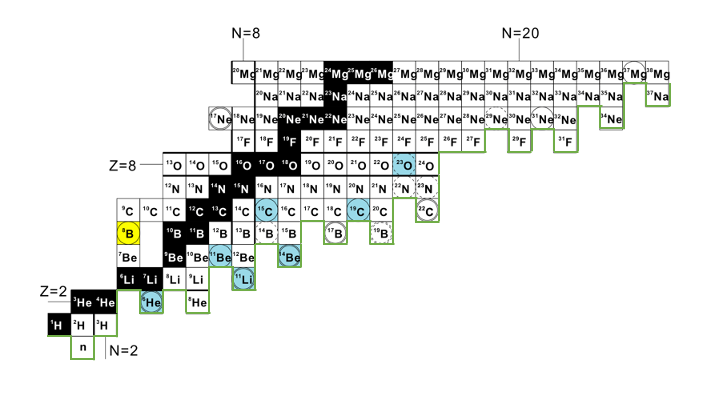
\includegraphics[width=14cm]{nuclear_chart.png}
    \caption{Nuclear Chart}
    \label{Nuclear chart}
\end{figure}
\begin{figure}
    \centering
    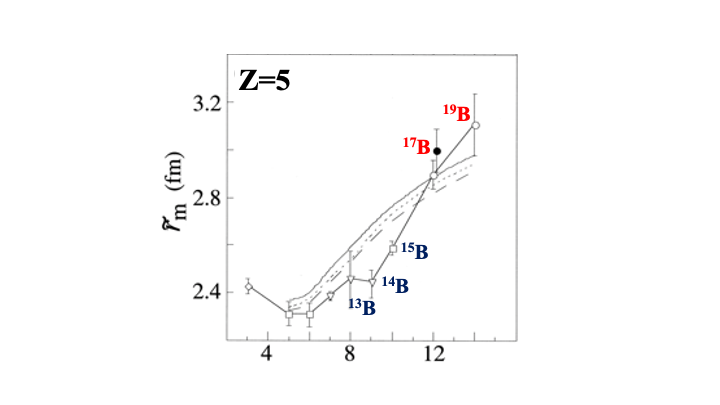
\includegraphics[width=14cm]{Radius_of_boron.png}
\end{figure}
2 중성자 헤일로로 알 수 있는 것은 dineutron에 대한 연구이다. 
본 논문에서는 납 타겟을 이용하여 17B를 Coulomb dissociation 시키고, 15B와 두 중성자를 검출하여 17B의 soft E1 Excitation을 조사하였다.


\chapter{Methods}

In this chapter, the methods used in this research are explained. First, Coulomb dissociation is introduced as a method to research the halo structure of $^{17}$B. For the part of it, equivalent photon method as a tool for investigating the soft $E1$ excitation of $^{17}$B is described. The $E1$ reduced transition probability $B(E1)$ and the geometrical information which is related to dineutron correlation can be obtained. Next, for extracting the Coulomb dissociation cross section from experimental data, the subtraction of nuclear breakup component is explained. Finally, the invariant mass method for the reconstruction of experimental data is explained. 

\section{Coulomb Dissociation}
\begin{figure}[t]
    \centering
    \setlength{\unitlength}{1mm}
    \begin{picture}(100,52)
        % Boron-17 nucleus
        \put(10,40){\circle{15}}
        \put(10,42){\circle{10}}
        \put(7,41){\footnotesize ${}^{15}$B}
        \put(8,35){\circle*{2}}
        \put(12,35){\circle*{2}}
        \put(8,30){\footnotesize n     n}
        \put(6,49){${}^{17}$B}

        % Arrow to excited state
        \put(20,40){\vector(1,0){20}}

        % Excited Boron-17 nucleus
        \put(50,40){\circle{15}}
        \put(50,42){\circle{10}}
        \put(47,41){\footnotesize ${}^{15}$B}
        \put(48,35){\circle*{2}}
        \put(52,35){\circle*{2}}
        \put(48,30){\footnotesize n      n}
        %\put(50,20){\line(0,-1){12}}
        \put(50,15){\circle{12}}
        \put(48,14){\footnotesize Pb}
        \put(46,49){${}^{17}$B$^*$}

        % Gamma ray
        \multiput(50,21)(0,1){7}{\line(0,1){0.5}}
        \multiput(50,9)(0,-1){7}{\line(0,-1){0.5}}
        \multiput(53,20)(0.4,1){7}{\line(0.4,1){0.2}}
        \multiput(47,20)(-0.4,1){7}{\line(-0.4,1){0.2}}
        \multiput(53,10)(0.4,-1){7}{\line(0.4,-1){0.2}}
        \multiput(47,10)(-0.4,-1){7}{\line(-0.4,-1){0.2}}

        %\multiput(50,15)(-3,3){5}{\line(0,-0.3){1}}
        \put(42,20){\footnotesize $\gamma$}

        % Arrow to final state
        %\put(60,20){\vector(1,0){20}}

        % Final state boron-15
        \put(90,47){\circle{10}}
        \put(87,45.5){\footnotesize ${}^{15}$B}
        \put(60,40){\vector(1,0.3){20}}
        \put(96,49){\footnotesize \( E_{^{15}\text{B}}, \vec{P}_{^{15}\text{B}} \)}

        % Final state neutron 1
        \put(90,33){\circle*{2}}
        \put(86,33.5){\footnotesize $n$}
        \put(60,40){\vector(1,-0.25){25}}
        \put(92,33){\footnotesize \( E_{n1}, \vec{P}_{n1} \)}
        % Final state neutron 2
        \put(90,28.5){\circle*{2}}
        \put(86,29){\footnotesize $n$}
        \put(60,40){\vector(1,-0.37){25}}
        \put(92,28){\footnotesize \( E_{n2}, \vec{P}_{n2} \)}

    \end{picture}
   \caption[Schematic representation of Coulomb dissociation]{Schematic representation of Coulomb dissociation of ${}^{17}$B. The ${}^{17}$B is induced to Pb target and excited by virtual photon made from electric magnetic field by relativistic movement between ${}^{17}$B and Pb target. The excited ${}^{17}$B is dissociated into ${}^{15}$B and two neutrons. The $E$ and $\vec{P}$ are represent total energy and momentum of each fragment respectively.}
   \label{fig:CD_drawing}
\end{figure}

Coulomb dissociation is breakup reaction from excited stated by Coulomb excitation. Figure \ref{fig:CD_drawing} shows the scheme of the Coulomb dissociation of ${}^{17}$B used in this research. When nuclei incident into the high-Z target like lead, the projectile is excited by the electric field of target. When the final state is above the decay threshold, the Coulomb dissociation occurs.

\subsection{Equivalent Photon Method}
Equivalent photon method\cite{Jackson}\cite{Bertulani}\cite{Aumann} is a powerful tool for investigating Coulomb excitation/dissociation in terms of the virtual photon. Under the equivalent photon method, Coulomb dissociation cross section $\sigma_{CD}$ can be described with the photon absorption cross section $\sigma_{\gamma}^{E1}(E_x)$ and the virtual photon number $N_{E1}(E_x)$ as
\begin{align}
    \frac{d\sigma_{CD}}{dE_x} = \frac{N_{E1}(E_x)}{E_x} \sigma_{\gamma}^{E1}(Ex),
\end{align}
where $E_x$ is the excitation energy of nuclei, $N_{E1}(E_x)$ is the virtual photon number produced by $E1$ transition. And the photon absorption cross section $\sigma_{\gamma}^{E1}$ can directly be related to the $E1$ reduced transition probability $dB(E1)/dE_x$ as
\begin{align}
    \sigma_{\gamma}^{E1} = \frac{16 \pi^3}{9 \hbar c} E_x \frac{dB(E1)}{dE_x}. \label{eq:photon_absorption}
\end{align}
Then, the Coulomb dissociation cross section is written as
\begin{align}
    \frac{d\sigma_{CD}}{dE_x} = \frac{16 \pi^3}{9 \hbar c} N_{E1}(E_x) \frac{dB(E1)}{dE_x}.
\end{align}
The virtual photon number for $E1$ transition $N_{E1}$ is obtained by investigating the photon flux at an impact parameter $b$ as
\begin{align}
    N_{E1}(E_x) &= \int_{b}^{\infty} 2\pi b n_{E1}(E_x, b) db  \\
                &=\frac{2}{\pi}Z^{2}_{1}\alpha\Big(\frac{c}{v}\Big)^{2}\Big[\xi K_{0}(\xi)K_{1}(\xi)-\frac{v^{2}\xi^{2}}{2c^{2}}(K^{2}_{1}(\xi)-K^{2}_{0}(\xi)\Big] \label{eq:Virtual_Photon}
\end{align}

\begin{adjustwidth}{1cm}{1cm}
    $\xi = E_x b / \gamma v \hbar$ \\
    $E_{\gamma} = \omega \hbar$ : Virtual photon energy\\ 
    $Z_{1}$ : Atomic number of target\\
    $b$ : Impact parameter 1.3 ($17^{1/3} + 208^{1/3}$) = 11.048 fm\\
    $K_0, K_1$ : Modified Bessel function of order zero and one \\
    $\alpha = e^2 / \hbar c$ : Fine structure constants\\
\end{adjustwidth}
%\vspace{1mm}
In this experiment, we assumed the virtual photon energy $E_{\gamma}$ is equal to excitation energy $E_x$ of projectile. In Figure \ref{fig:Virtual_Photon}, the virtual photon number $N_{E1}(E_x)$ for $E1$ transition in the function of excitation energy $E_x$ and the reduced $E1$ transition probability $dB(E1)/dE_x$ corresponding to energy region are shown. You can see there are two peaks corresponding to soft $E1$ excitation and giant dipole resonance respectively. Since the virtual photon number is exponentially decreasing with the excitation energy, the equivalent photon method is best suited for investigating the excitation in low energy region. 

\begin{figure}[t]
    \centering
    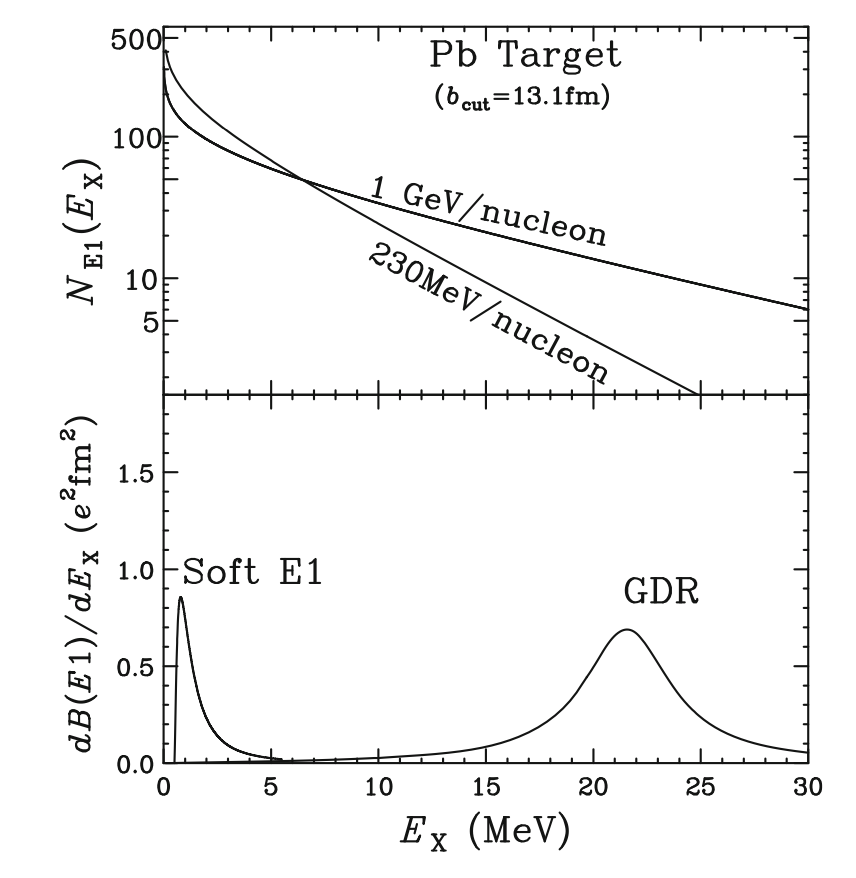
\includegraphics[width=8cm]{chapter2/Virtual_Photon.png}
    \caption[Virtual photon number $N_{E1}(E_x)$ spectra and $dB(E1)/dE_x$ spectrum for halo nucleus\cite{Nakamura23}]{Virtual photon number $N_{E1}(E_x)$ spectra with the $dB(E1)/dE_x$ spectrum for halo nucleus\cite{Nakamura23}. The peak near 1 MeV shows the soft $E1$ excitation, while the peak in high energy region ($\sim 20$ MeV) represents the giant dipole resonance.}
    \label{fig:Virtual_Photon}
\end{figure}

\subsection{Geometry of Two Neutron Halo and Dineutron Correlation}
Another information which can be extracted from $E1$ reduced transition probability is related with the geometrical value of the two neutron halo nucleus. By non-energy weighted cluster sum rule from Esbensen et at. \cite{Esbensen}, the $E1$ reduced transition probability $B(E1)$ in entire energy region can be written as 
\begin{align}
    B(E1) &= \int_{-\infty}^{\infty} \frac{dB(E1)}{dE_x}dE_x \notag \\
        &= \frac{3}{\pi} \bigg(\frac{Z e}{A}\bigg)^2 \langle r^2_{c-nn} \rangle,
        %&= \frac{3}{4 \pi} \bigg(\frac{Z e}{A}\bigg)^2 \langle \vec{r_1}^2 + \vec{r_2}^2 + 2 \vec{r_1} \cdot \vec{r_2} \rangle \notag \\
        %&= \frac{3}{4 \pi} \bigg(\frac{Z e}{A}\bigg)^2 \langle \vec{r_1}^2 + \vec{r_2}^2 + 2\vec{r_1} \vec{r_2} \cos \theta_{nn} \rangle
\end{align}
where $\langle r^2_{c-nn} \rangle$ is a root mean square (rms) distance between the core nucleus and the two center of mass of two neutron. Furthermore, the distance between two neutrons $\langle r^2_{nn} \rangle$ can be obtained from matter radius of halo and core nucleus in the three body model as \cite{Bertulani07}\cite{Hagino07},
\begin{align}
    \langle r^2_{m} \rangle = \frac{A_c}{A} \langle r^2_{m} \rangle_{c} + \frac{2A_c}{A^2} \langle r^2_{c-nn} \rangle + \frac{1}{2A} \langle r^2_{nn} \rangle
\end{align}
where $A$ and $A_c (= A - 2)$ are the mass number of halo and core nucleus respectively. $\langle r^2_{m} \rangle$ and $\langle r^2_{m} \rangle_{c}$ are the matter radius of halo and core nucleus respectively. In this research, for calculation, we use the value $\langle r^2_{m} \rangle = 3.00 (6)$ fm, $\langle r^2_{m} \rangle_c = 2.75 (6)$ fm from the rms radius of $^{17}$B and $^{15}$B respectively \cite{Estrade}. $\langle r^2_{nn} \rangle$ is the distance between two neutrons.
Finally, the opening angle between two neutrons $\langle \theta_{nn} \rangle$ can be obtained as,
\begin{align}
    \cos \frac{\theta_{nn}}{2} = \frac{r_{c-nn}}{\sqrt{r^2_{c-nn} + \frac{r^2_{nn}}{4}} }.
\end{align}


\section{Contribution of Nuclear Breakup}
For evaluating the $B(E1)$ value, we need to extract only the Coulomb dissociation component from the experimental data. In this research, we used $\Gamma$ factor method to remove the contribution of nuclear breakup component from lead target. For extracting the Coulomb dissociation cross section $\sigma(CD)$, we subtract the reaction cross section with the carbon target scaled by $\Gamma$ factor from the one with the lead target. Using this method, we can write the Coulomb dissociation cross section as follows.
\begin{align}
    \sigma_{CD} = \sigma(\text{Pb}) - \Gamma \sigma(\text{C}),\label{eq:CD}
\end{align}
$\sigma(\text{C})$ and $\sigma(\text{Pb})$ are the reaction cross section with carbon and lead target respectively. $\Gamma$ is the ratio of the reaction cross section with lead target to the one with carbon target. The $\Gamma$ factor can be obtained from the geometry between the projectile and target nucleus as,
\begin{align}
    \Gamma_{\text{min}} &= \frac{R_{\text{Pb}} + R_{{}^{17}\text{B}}}{R_{\text{C}} + R_{{}^{17}\text{B}}} = \frac{A_{\text{Pb}}^{1/3} + A_{^{17}\text{B}}^{1/3}}{A_{\text{C}}^{1/3} + A_{^{17}\text{B}}} = 1.75\\
    \Gamma_{\text{max}} &= \frac{R_{\text{Pb}}}{R_{\text{C}}} = \frac{A_{\text{Pb}}^{1/3}}{A_{\text{C}}^{C}} = 2.59
\end{align}
In this experiment, we used $\Gamma = 2.835$ value from calculation including the consideration of incident energy of $^{17}$B at the middle of target (270 MeV/u)\cite{Ogata}.

\section{Invariant Mass Method}
To reconstruct the excited state of ${}^{17}$B at target, invariant mass method is used. Since ${}^{17}$B has no bound excited state and its two neutron separation energy $S_{2n}$ is very small, the dissociation process occurs very quickly. In this case, the invariant mass method is a useful tool to reconstruct the intermediate excited state of the system by measuring the momentum and energy of all of the fragments. The invariant mass of the excited state $M^{*}$ is defined as
\begin{align}
    M^* &= \sqrt{\bigg(\sum_{i} E_i\bigg)^2 - \bigg(\sum_{i}\vec{P}_i \bigg)^2} 
\end{align}
where $E_i$ and $\vec{P}_i$ are the energy and momentum of the fragment $i$ respectively. In this experiment, the excited state of ${}^{17}$B is reconstructed by measuring the momentum and energy of ${}^{15}$B and two neutrons. The relative energy $E_{rel}$ between ${}^{15}$B and two neutron can be written with the invariant mass as
\begin{align}
    E_{rel} &= M({}^{17}\text{B}^*) - (m_{{}^{15}\text{B}} + m_n + m_n)
\end{align}
where $m_{{}^{15}\text{B}}$, $m_n$ and $m_n$ are the mass of ${}^{15}$B and two neutrons respectively. The relative energy $E_{rel}$ is related to the excitation energy $E_x$ of ${}^{17}$B and neutron separation energy $S_{2n}$ as
\begin{align}
    E_{rel} &= E_x - S_{2n}
\end{align}
Figure \ref{fig:Invariant_Mass} shows the schematic representation of the invariant mass method. 

\begin{figure}[t]
    \centering
    \setlength{\unitlength}{1mm}
    \begin{picture}(60,40)
        \put(6,15){$E_x$}
        \put(16,1){${}^{17}$B}
        \put(18,31){$M^*$}
        \put(49,11){${}^{15}$B + n + n}
        \put(29,18){$E_{rel}$}
        \put(33,4){$S_{2n}$}
        %\put(10,0){\dashbox{dash-len}}}
        \thicklines
        \put(10,30){\line(1,0){20}}
        \put(10,0){\line(1,0){20}}
        \put(50,10){\line(1,0){20}}
        \put(20,5){\vector(0,1){24}}
        \put(31,29){\vector(1,-1){18}}
        \thinlines
        \multiput(26,10)(1.2,0){20}{\line(1,0){0.8}}
        \multiput(28,0)(1.2,0){10}{\line(1,0){0.8}}
        \put(28,20){\vector(0,1){10}}
        \put(28,20){\vector(0,-1){10}}
        \put(12,20){\vector(0,1){10}}
        \put(12,20){\vector(0,-1){20}}
        \put(32,5){\vector(0,1){5}}
        \put(32,5){\vector(0,-1){5}}
        
    \end{picture}
    \caption{Schematic representation of the invariant mass method} 
    \label{fig:Invariant_Mass}
\end{figure}
\chapter{Experiment}
    This chapter describes about experimental setup in this study. The experiment is performed at Rare Isotope Beam Factory (RIBF) at RIKEN Nishina Center.\cite{RIKEN} A primary ${}^{48}$Ca beam is produced by the RIKEN accelerator complex and delivered to the BigRIPS separator. \cite{Kubo03} \cite{Kubo07} \cite{Kubo12} The BigRIPS separator produced the ${}^{17}$B secondary beam which bombarded on the lead and carbon targets in front of the SAMURAI (Superconducting Analyzer for MUlti-particles from Radioisotope beams) spectrometer. \cite{SAMURAI} After the reaction at target, the fragments ${}^{15}$B and two neutrons are detected by detectors at SAMURAI area. Note that this experiment was part of the SAMURAI Dayone experiment which was the first physics run using the SAMURAI spectrometer.

\section{BigRIPS separator}

    \begin{figure}
        \centering
        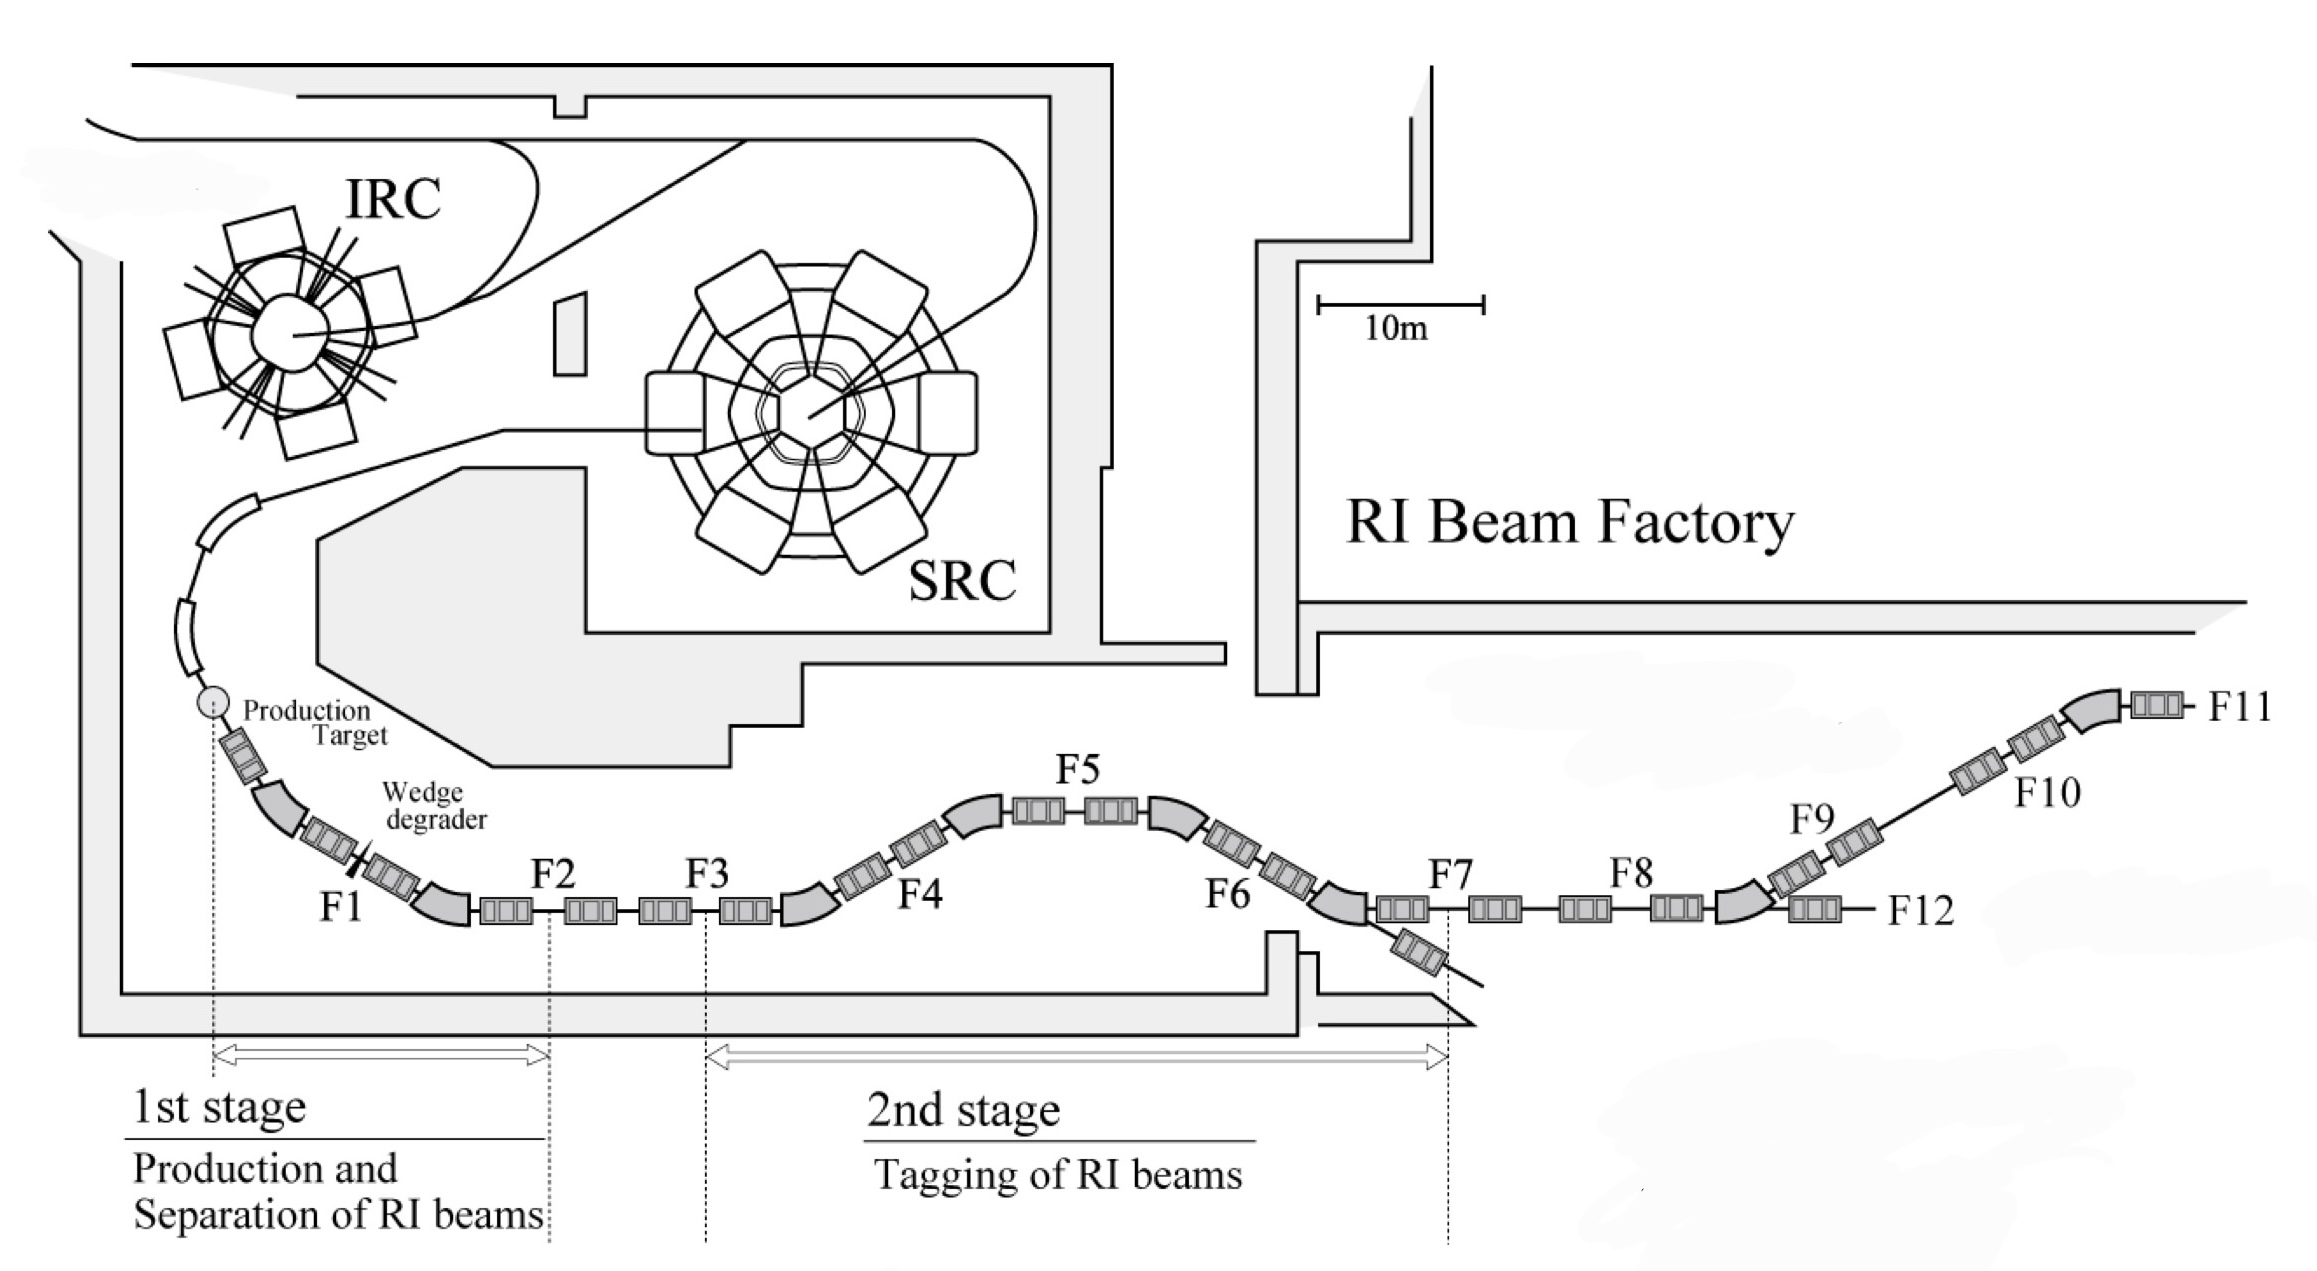
\includegraphics[width=12cm]{chapter3/BigRIPS_roof.jpg}
        \caption{A top view of the BigRIPS separator}
    \end{figure} 

After primary ${}^{48}$Ca beam is produced at SRC accelerator, the beam bombarded on a 30mm thick Be target and the secondary beam is produced through the in-flight fragmentation method. Since the secondary beam includes many rare isotopes, the RI beam is separated by the BigRIPS separator. Table 3.1 shows the BigRIPS separator setup for Dayone experiment. In the first stage of BigRIPS separator, the RI beam separated by dipole magnet with slit and wedge-shaped degrader located at F1 focal plane. In the dipole magnet, the rigidity of a particle can be written as following eq \ref{eq:rigidity}.
    \begin{align}
        \rho = \frac{A}{Z} \cdot\frac{v}{B} \label{eq:rigidity}
    \end{align}
The velocity of the secondary beam is almost same regardless of the nuclei so that it can be possible to choose specific $A/Z$ by adjusting the slit to filter only some $B\rho$ value. After that, the wedge-shaped degrader makes the beam energy depends on the $Z$ so that even same $A/Z$ nuclei can be separated. In the second stage, the RI beam is identified using TOF-B$\rho$-$\Delta E$ method. Each detector information will be described as following.
    \begin{table}[h]
        \centering
        \begin{tabular}{c c c c}
            \hline
            Focal Plane & Dipole Magnet [Tm] & Slit[mm] & Degrader / Detector \\
            \hline
            F0  & 9.1734 &  & Be target (30mm) \\
            F1  & 8.8195 & $\pm$120 & Al wedge degrader \\
            F2  & 8.8195 & L: 10 R: 7 & \\
            F3  & 8.7841 &  & Plastic Scintillator (3mm)\\
            F5  & 8.780  & $\pm$120 & BPC \\
            F7  & 8.780  & $\pm$120 & Plastic Scintillator (3mm)\\
            %F13 &  & & Plastic Scintillator (0.5mm$\times$2)\\
            \hline
        \end{tabular}
        \caption{BigRIPS separator setup for Dayone experiment \cite{Dayonelog}}
    \end{table}

\subsection{Plastic Scintillator}
At focal plane F3, F7, F13, plastic scintillators are located for measuring the time of flight (TOF) of secondary beam. In F3 and F7, plastic scintillator with 3mm thickness is located and at F13 there are two scintillators, SBT1 and SBT2, with 0.5mm thickness. The flight length between F7 and F13 (Average point of SBTs) is 3662.00mm.

\begin{table}[h]
    \centering
    \begin{tabular}{c|ccc}
        \hline
        & Location & Thickness & Distance from target upstream \\
        \hline
        SF3 & F3 & 3mm & 86053.56 mm\\
        SF7 & F7 & 3mm & 39483.58 mm\\
        SBT1 & F13 &0.5mm & 2904.08 mm\\
        SBT2 & F13 &0.5mm & 2824.08 mm\\
        \hline
    \end{tabular}
    \caption{Information of Plastic Scintillators at F3, F7, F13}
\end{table}


\subsection{BPC (Beam Proportional Chamber)}
BPC is Multi Wire Proportional Chamber (MWPC) located at F5 focal plane which is used for measuring the position of beam. The purpose of BPC is tagging magnetic rigidity and momentum of secondary beam.
\begin{table}[h]
    \centering
    \begin{tabular}{l|c}
        \hline
        Effective Area & (H)240mm x (V)150mm \\
        Configuration & $XX$ (2 Planes) \\
        number of wire & 64 $\times$ 2 = 128 \\
        Wire Pitch & 4mm \\
        Gas & $i$--${C}_{4} {H}_{10}$ at 50 torr\\
        \hline
    \end{tabular}
    \caption{Parameter of BPC (Beam Proportional Chamber) \cite{SAMURAI}}
\end{table}


\begin{figure}[h]
    \centering
    \begin{subfigure}[h]{\textwidth}
        \centering
        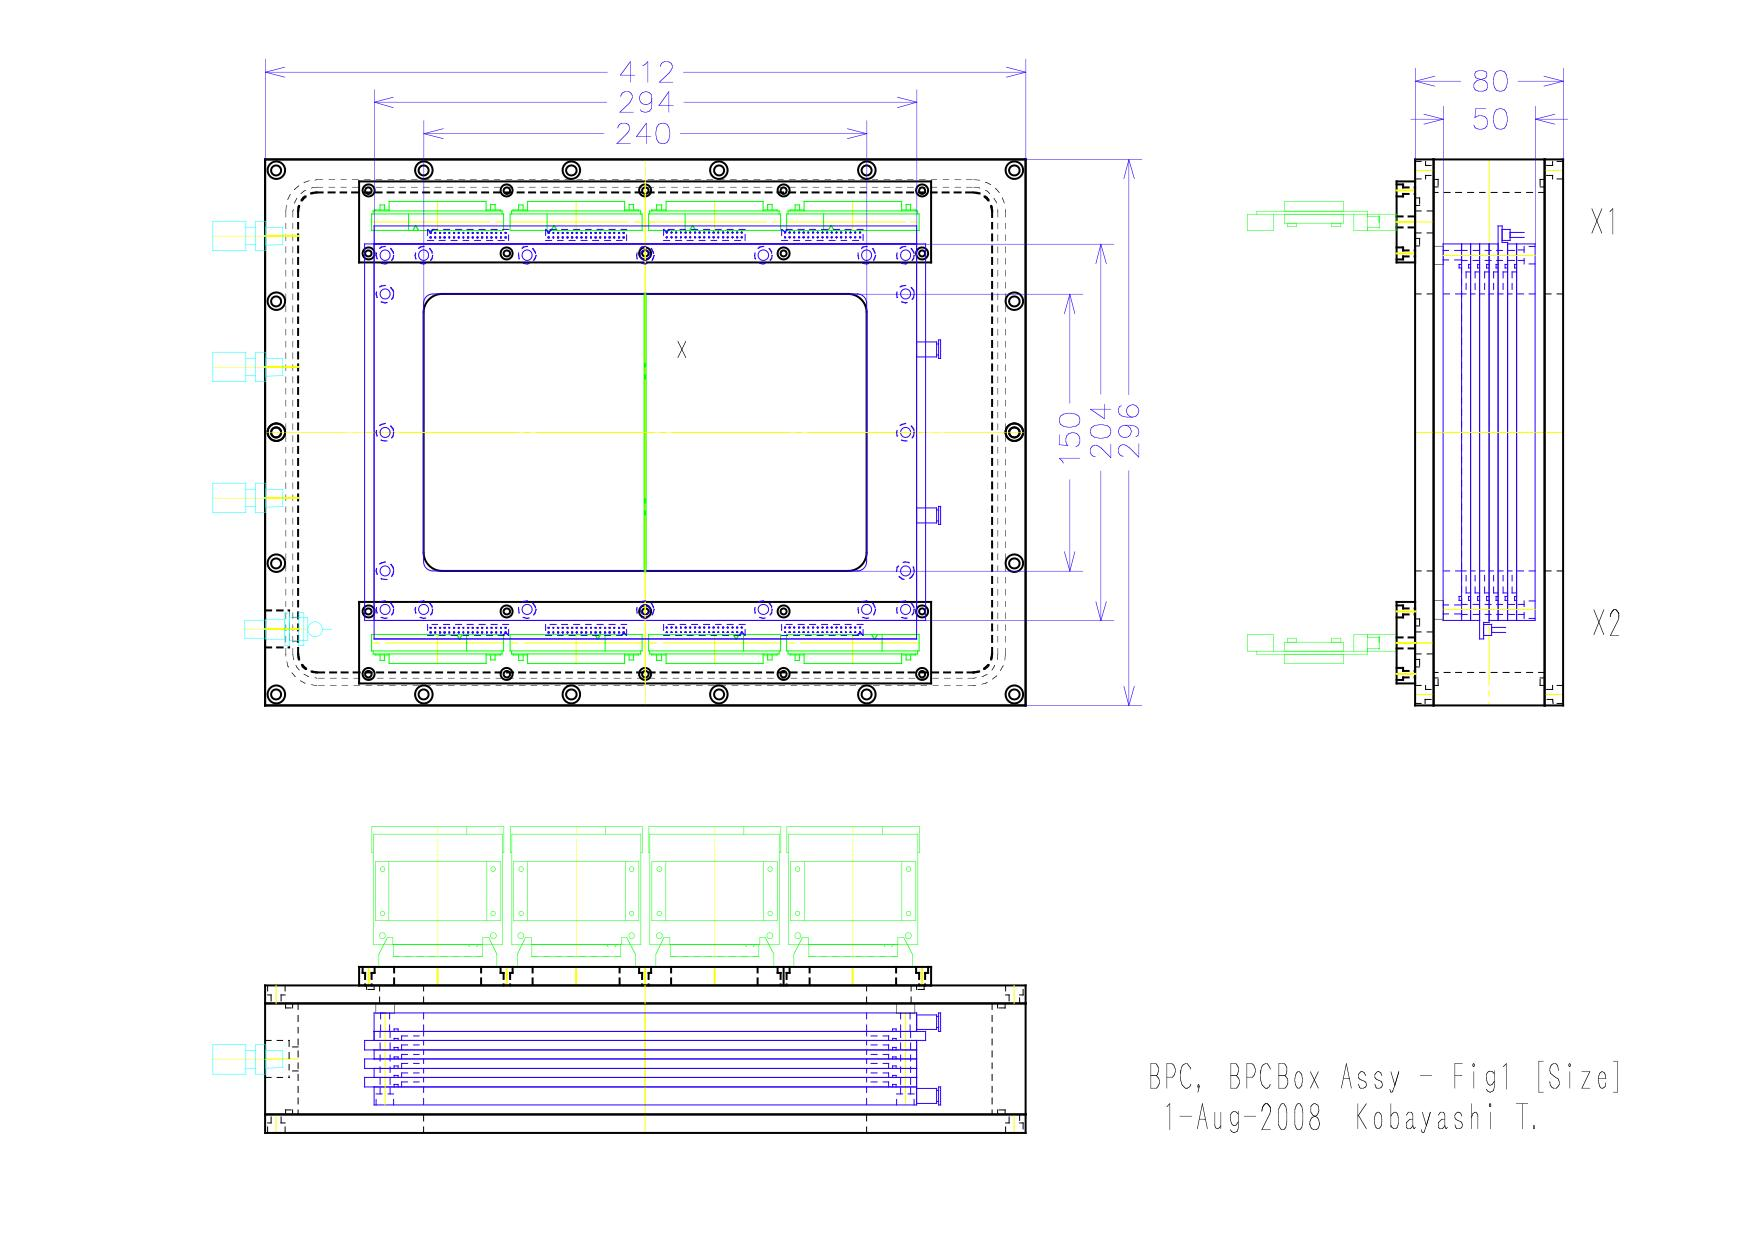
\includegraphics[width=12cm]{chapter3/bpc_a1.jpg}
    \end{subfigure}
    \begin{subfigure}[h]{\textwidth}
        \hspace{2.4cm}
        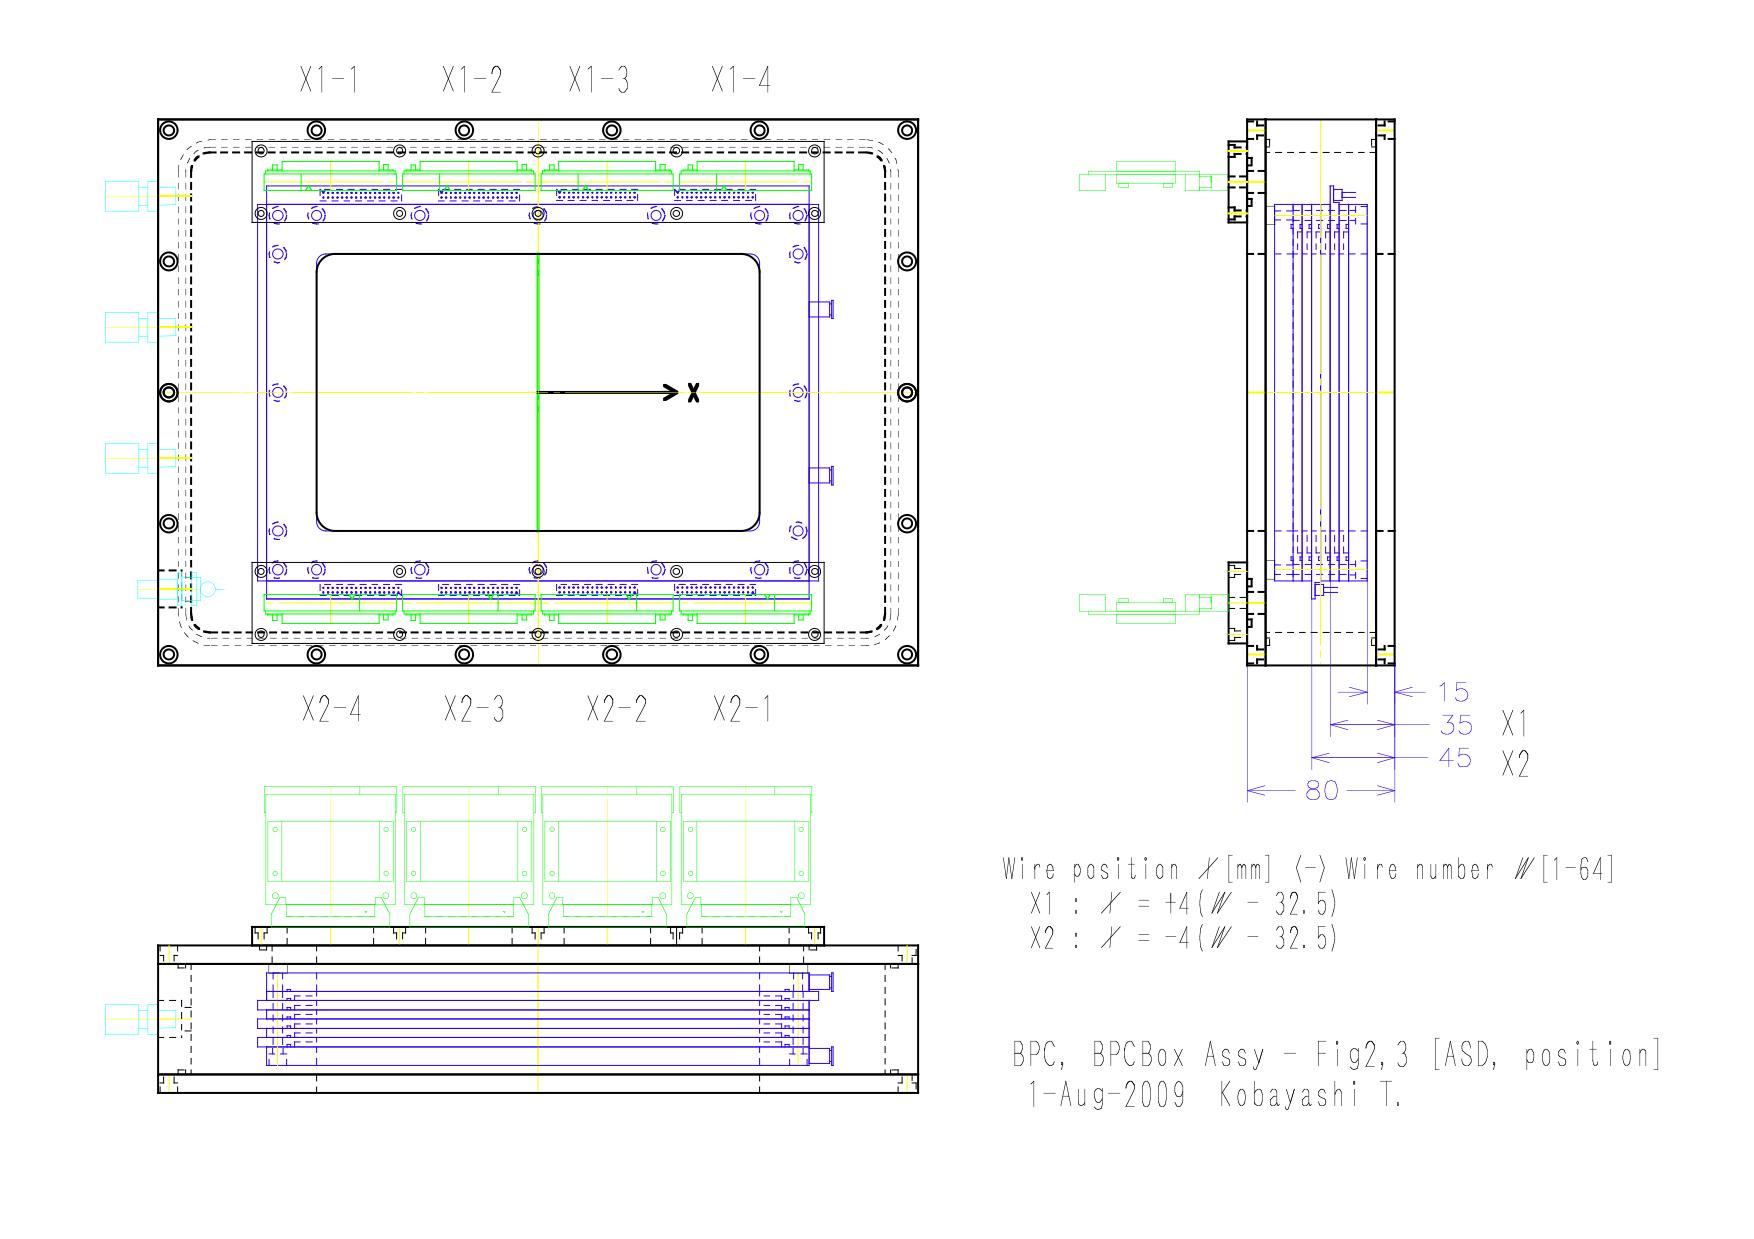
\includegraphics[width=12.5cm]{chapter3/bpc_a23.jpg}
    \end{subfigure}
        \caption{Schematic View of BPC (Beam Proportional Chamber) \cite{SAMURAI}}
\end{figure}

\clearpage

\subsection{ICB (Ion Chamber for Beam)}
The ICB is multi-layer ionization chamber for measuring the energy loss ($\Delta E$) of secondary beam. Using P10 gas at 1 atm, the energy loss of secondary beam can be measured. 
\begin{table}[h]
    \centering
    \begin{tabular}{l|c}
        \hline
        Effective Area & (H)140mm x (V)140mm x (D)420mm\\
        Configuration & 10 anodes and 11 cathodes \\
        Anode-cathode gap & 21mm \\
        Gas & P10 at 1 atm\\
        Distance from target upstream & 476.87 mm \\
        \hline
    \end{tabular}
    \caption{Parameter of ICB (Ion Chamber for Beam) \cite{SAMURAI}}
\end{table}

\begin{figure}[t]
    \centering
    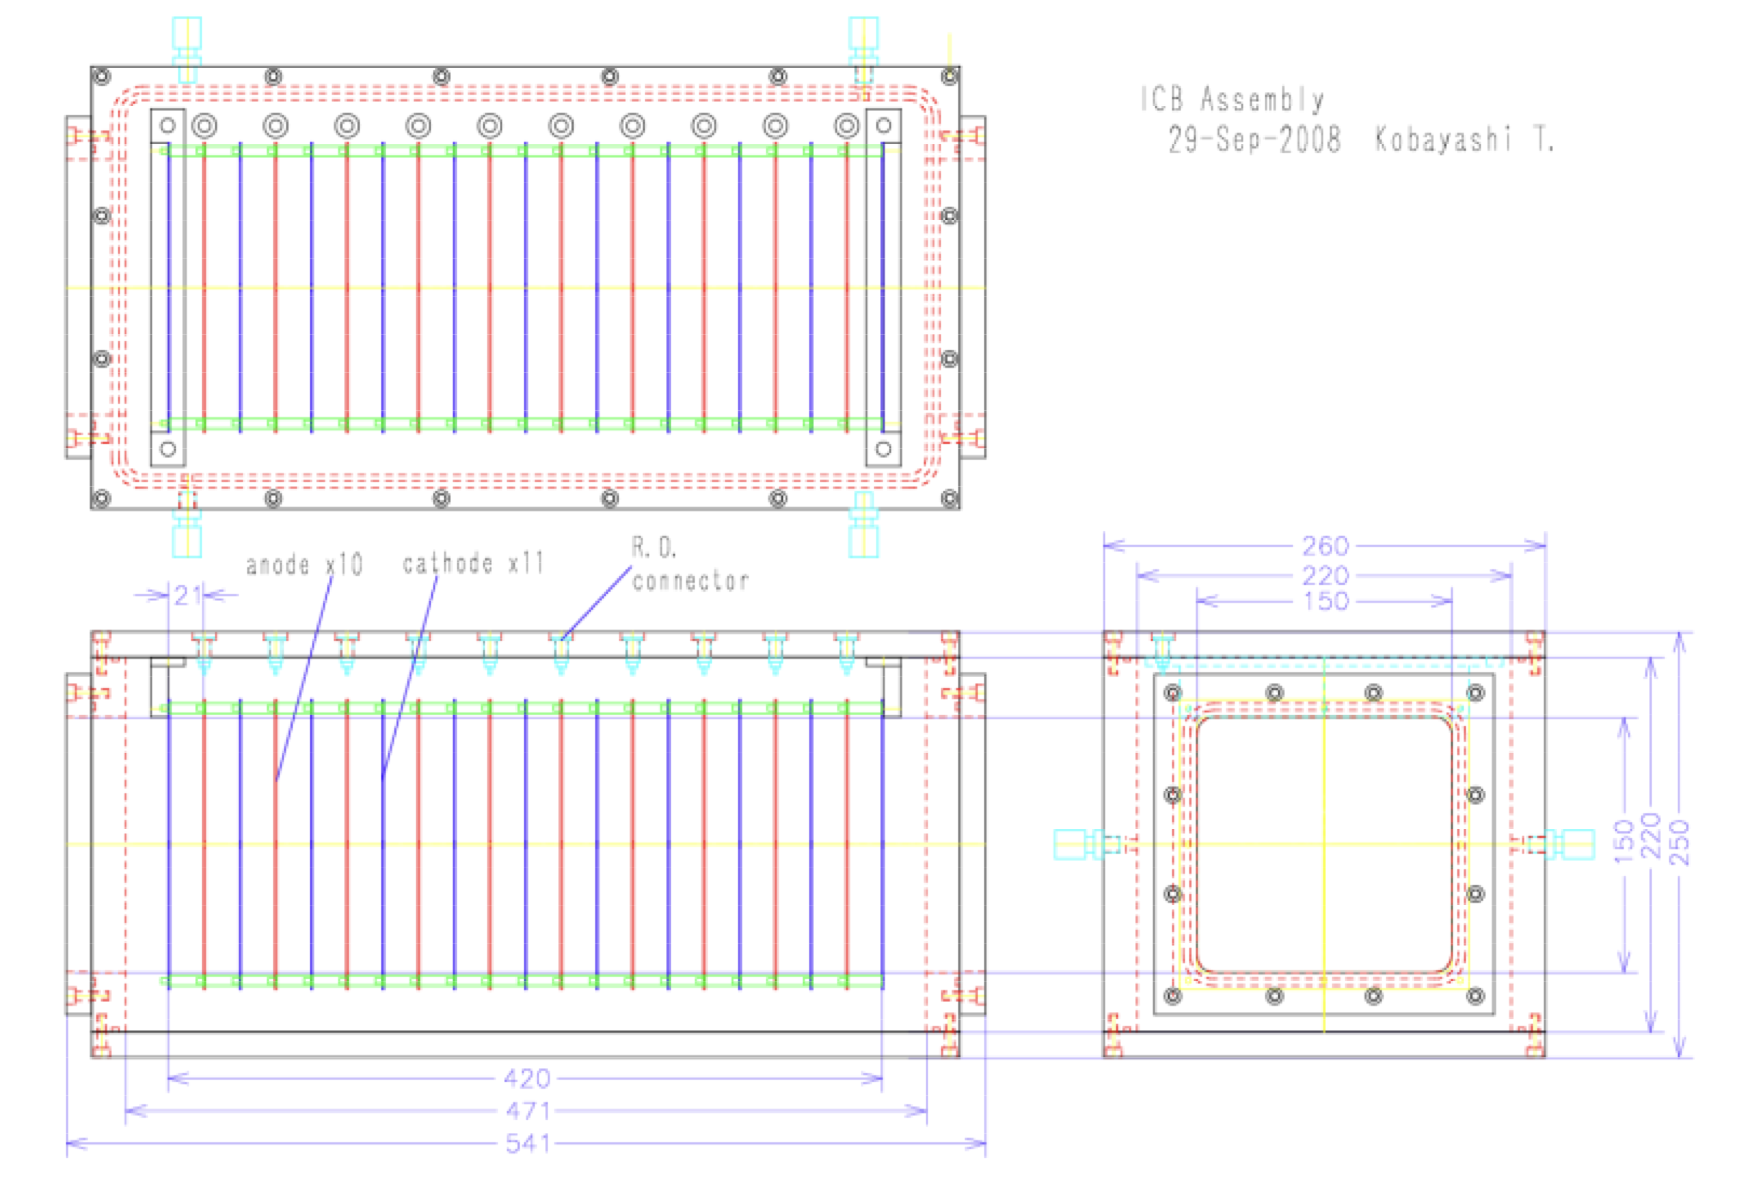
\includegraphics[width=11cm]{chapter3/icb_a}
    \caption{Schematic View of ICB (Ion Chamber for Beam) \cite{SAMURAI}}
\end{figure}

\subsection{BDC1, BDC2 (Beam Drift Chamber)}
Before target, there are two Beam drift chamber for reconstructing the trajectory of secondary beam. Using the trajectory information, the position of secondary beam at target can be calculated. In this experiment, each BDC box is filled with $i$--${C}_{4} {H}_{10}$ gas at 100 torr. 

\begin{table}[h]
    \centering
    \begin{tabular}[h]{l|c}
        \hline
        Effective Area & (H)80mm x (V)80mm\\
        Configuration & $XX'YY'XX'YY'$ (8 planes)\\
        Number of Wire & 16 $\times$ 8 = 128 \\
        Wire Pitch & 5mm \\
        Gas & $i$--${C}_{4} {H}_{10}$ at 100 torr\\
        Distance from target upstream & (BDC1) 2032.12mm (BDC2) 1032.8 mm \\
        \hline
    \end{tabular}
    \caption{Parameter of BDC (Beam Drift Chamber) \cite{SAMURAI}}
\end{table}

\begin{figure}[h]
    \centering
    \begin{subfigure}{\textwidth}
        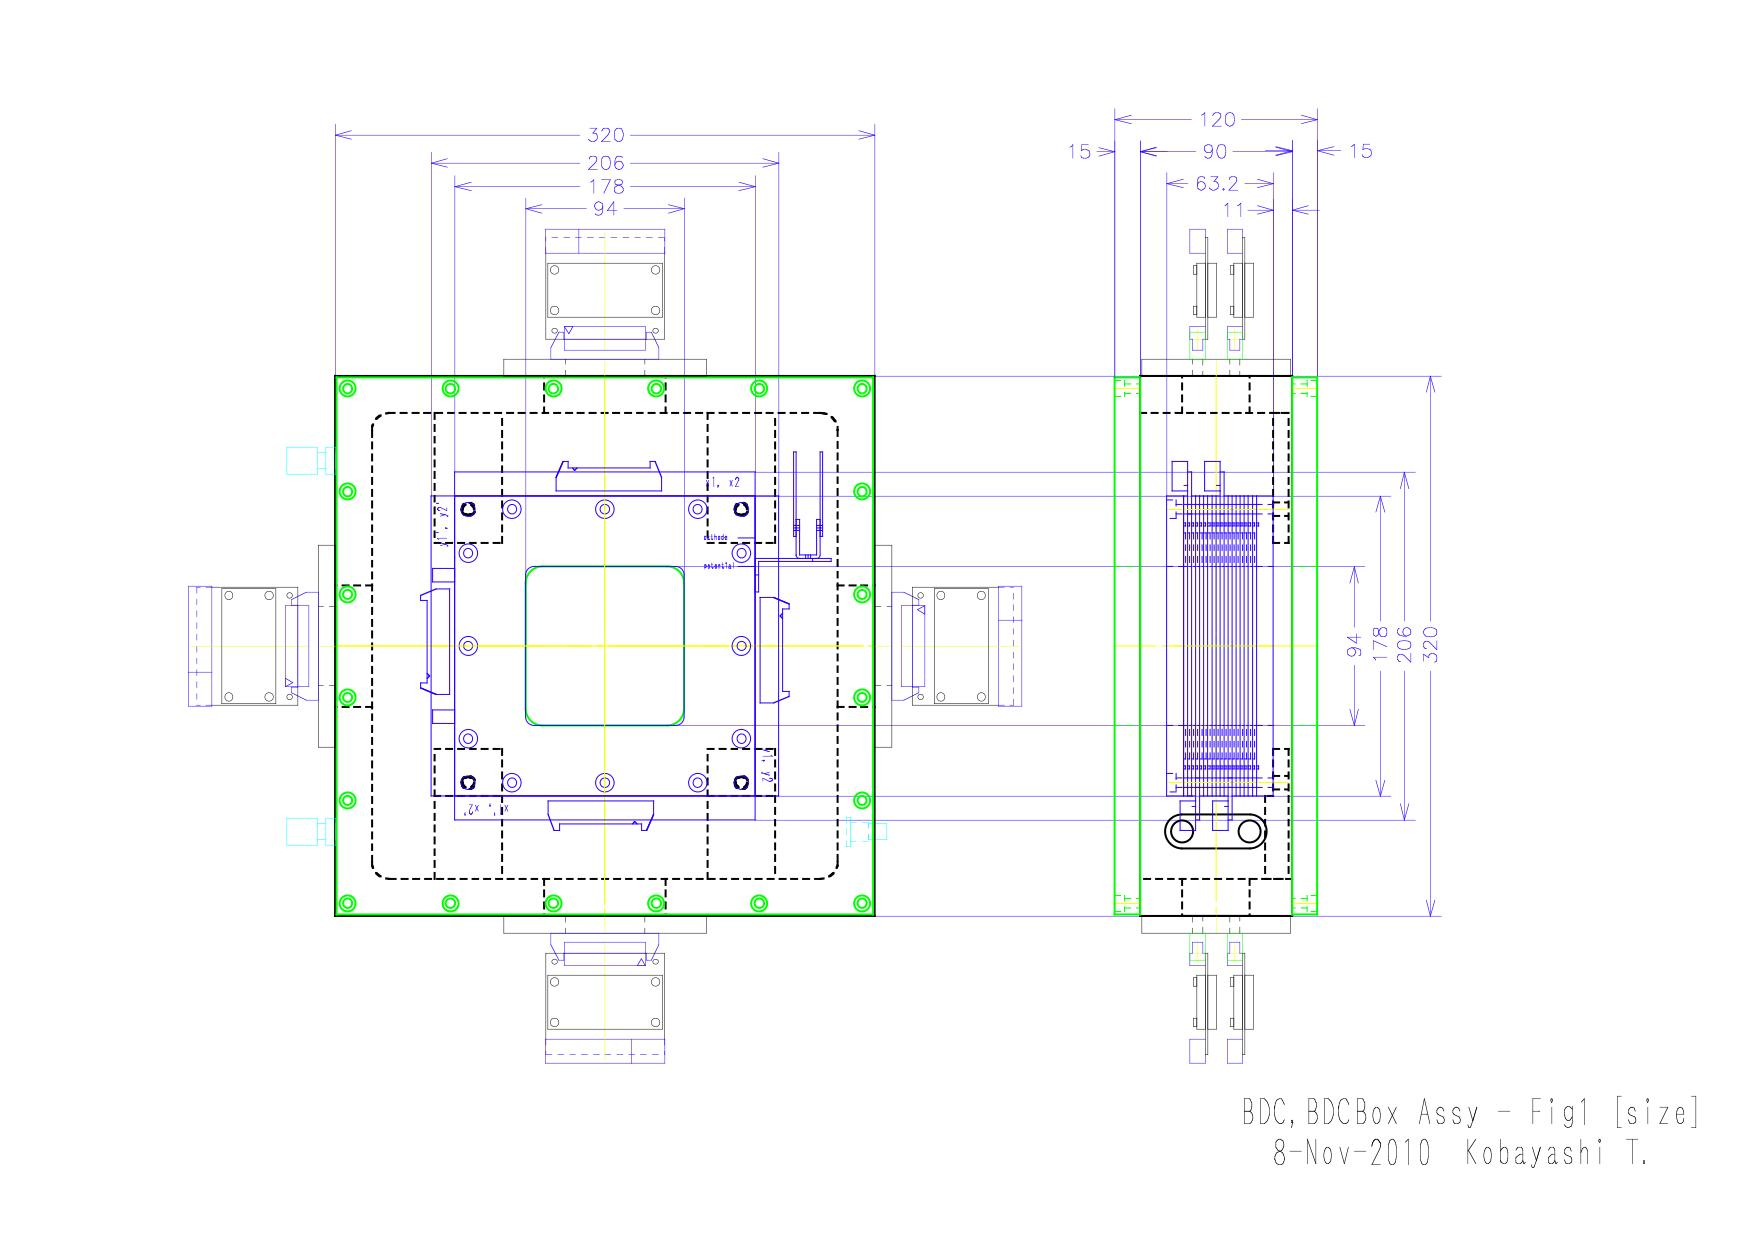
\includegraphics[width=12cm]{chapter3/bdc_a1.jpg}    
    \end{subfigure}
    \begin{subfigure}{\textwidth}
        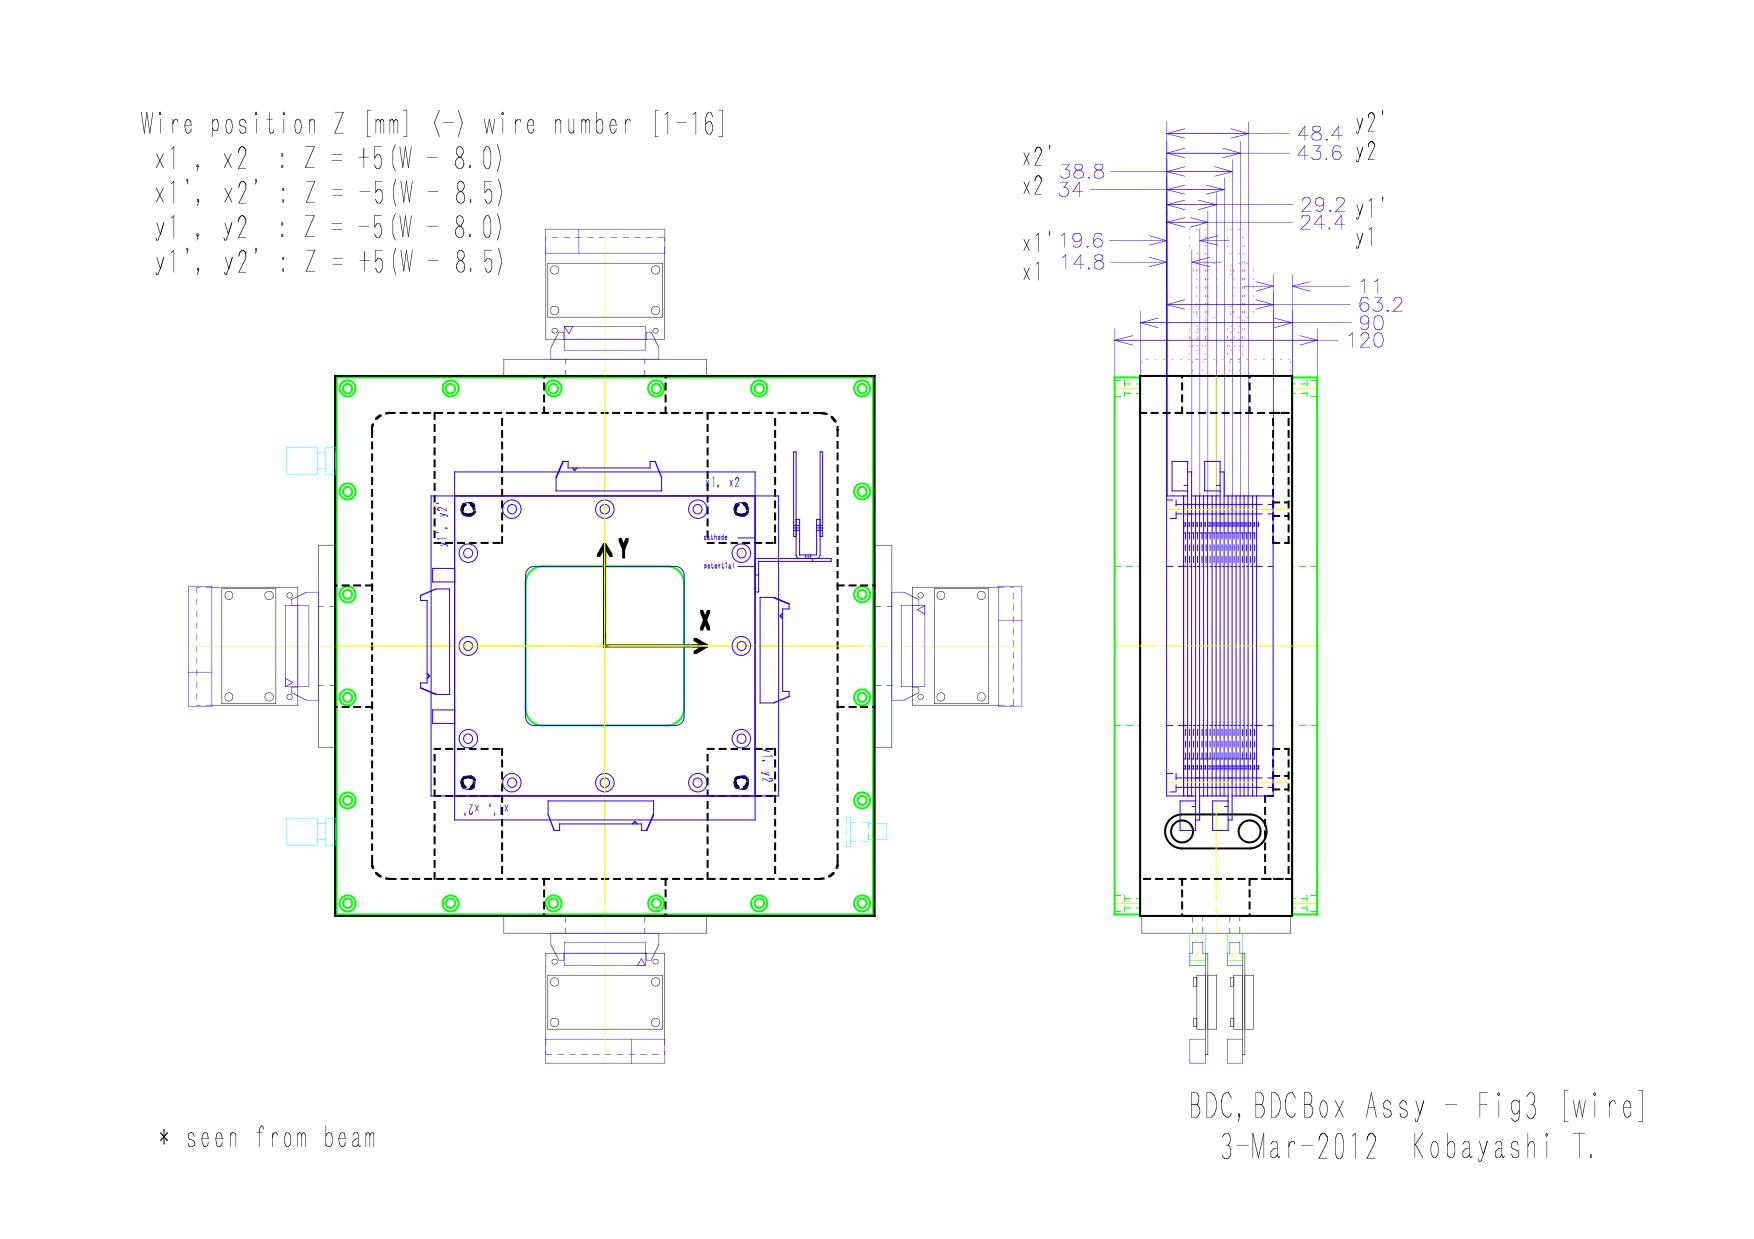
\includegraphics[width=12cm]{chapter3/bdc_a3.jpg}
    \end{subfigure}
    \caption{Schematic View of BDC (Beam Drift Chamber) \cite{SAMURAI}}
\end{figure}

\clearpage

\section{SAMURAI}

\begin{figure}[hbt!]
    \centering
    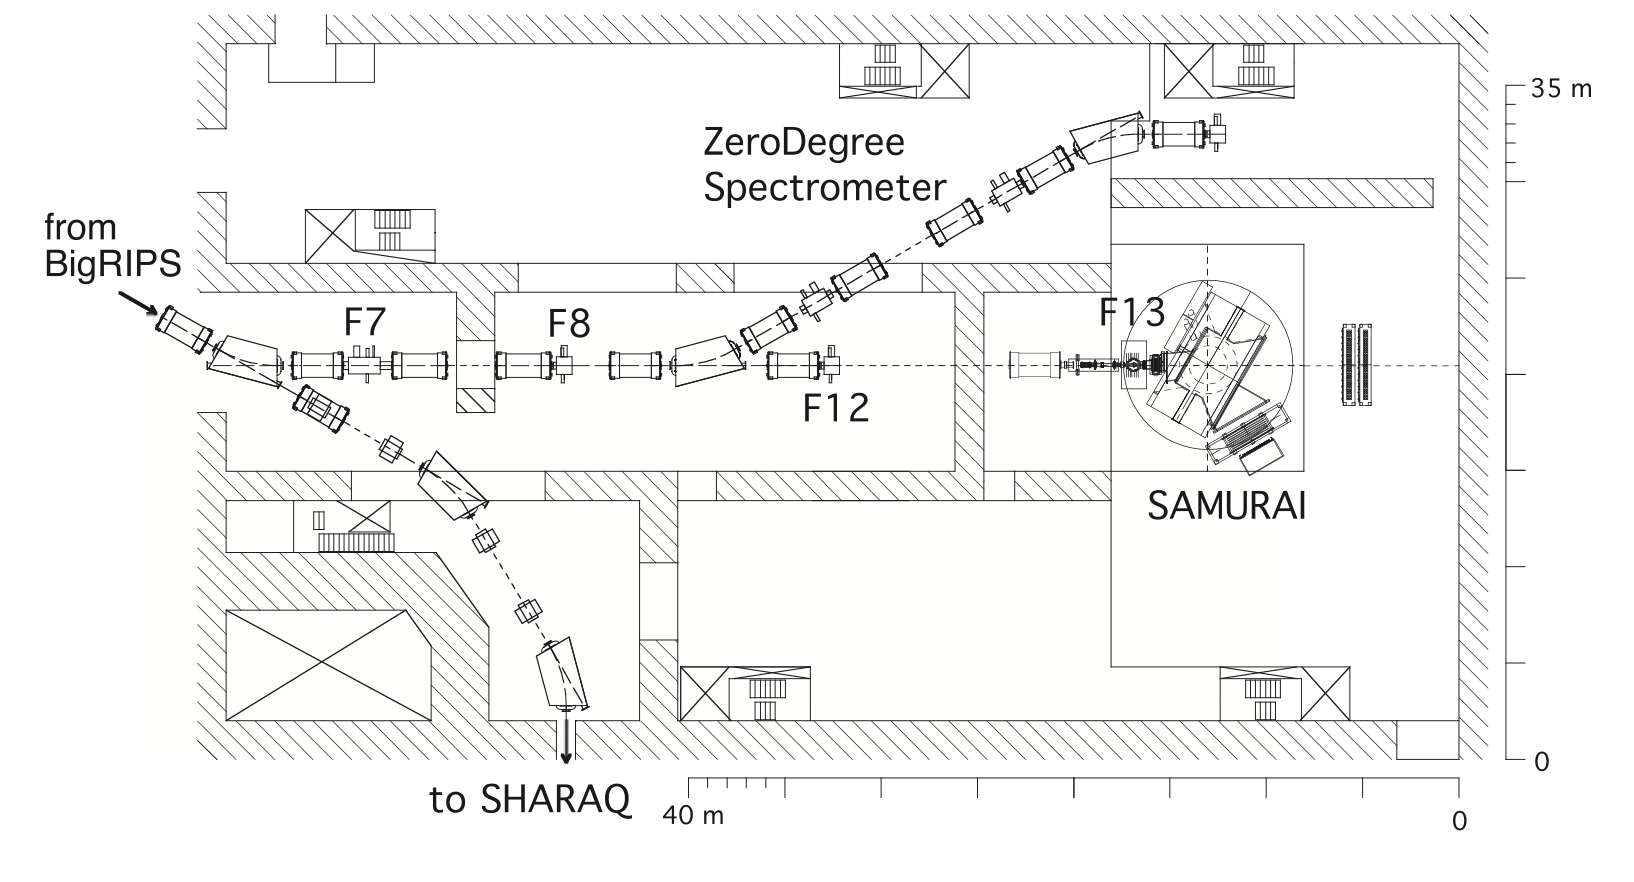
\includegraphics[width=12cm]{chapter3/SAMURAI1.png}
    \caption{A top view of the beam line from BigRIPS to SAMURAI spectrometer}
\end{figure}

The SAMURAI spectrometer is designed for kinematically complete experiment such as invariant mass spectroscopy. \cite{SAMURAIConcept} Charged fragment bent by SAMURAI superconducting magnet and detected by two drift chambers (FDC1, FDC2) and one plastic scintillator (HODF). Two drift chamber for fragment are located at before and after SAMURAI magnet, for rigidity analysis. And plastic scintillator HODF is placed after FDC2 to measure the TOF and energy loss of fragment. Finally the neutron detector array NEBULA is located at the end of extended beam line for neutron detection. Using SAMURAI system, the invariant mass of the system can be reconstructed by measuring all of the fragments and neutrons.

\begin{figure}[t]
    \centering
    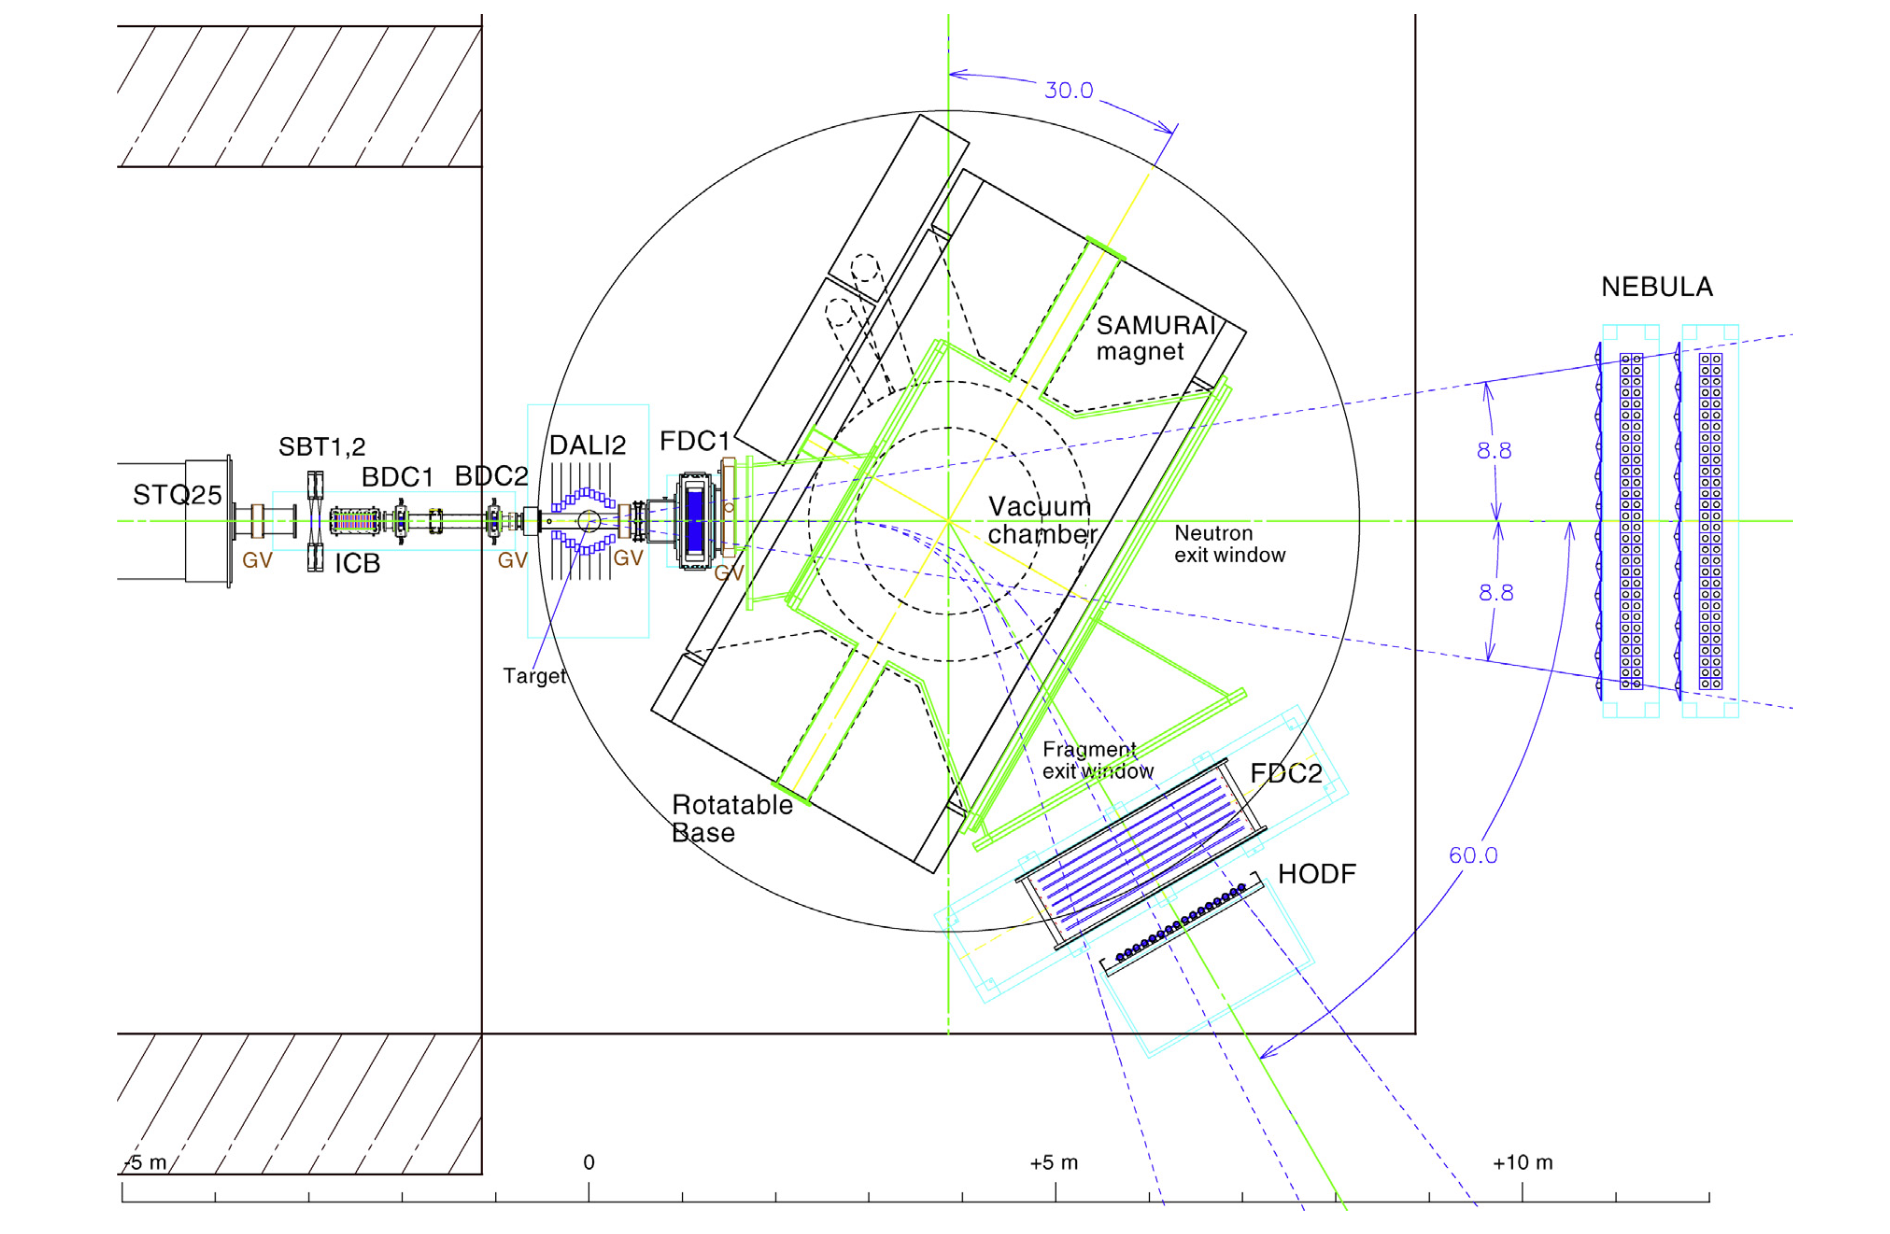
\includegraphics[width=12cm]{chapter3/SAMURAI.png}
    \caption{A top view of the SAMURAI spectrometer}
\end{figure}

\subsection{SAMURAI Magnet}

\begin{table}[h]
    \centering 
    \begin{tabular}{l|c}
    \hline
    Type & Superconducting dipole magnet \\
    Magnet Pole & $\phi$ 2m (0.88 m gap) \\
    Maximum field & 3.1 T \\
    Maximum current & 563 A \\
    Acceptance & $\theta_H \leq \pm 10{}^{\circ}$, $\theta_V \leq \pm 5{}^{\circ}$\\
    \hline
    \end{tabular}
    \caption{Parameter of SAMURAI Magnet \cite{SAMURAI}}
\end{table}

\subsection{FDC1, FDC2 (Forward Drift Chamber)}
After target, there are two Forward Drift Chamber for reconstructing the trajectory of charged fragment. Using the trajectory information, the rigidity of charged fragment at target can be calculated. In this experiment, FDC1 is filled with $i$--${C}_{4} {H}_{10}$ gas at 50 torr and FDC2 is filled with He + 50\% ${C}_{2} {H}_{6}$ gas at 1 atm. 

\begin{table}[h]
    \centering
    \begin{tabular}{l|c}
        \hline
        Effective Area & (H)400mm x (V)300mm x (D)180mm\\
        Configuration & $XX'UU'VV'XX'UU'VV'XX'$ (14 planes)\\
        Number of Wire & 32 $\times$ 14 = 448 \\
        Wire Pitch & 10mm \\
        Gas & $i$--${C}_{4} {H}_{10}$ at 50 torr\\
        Distance from target upstream & 1151.38 mm  \\
        \hline
    \end{tabular}
    \caption{Parameter of FDC1 (Forward Drift Chamber 1) \cite{SAMURAI}}
\end{table}

\begin{table}[h]
    \centering
    \begin{tabular}{l|c}
        \hline
        Effective Area & (H)2296mm x (V)836mm x (D)860mm\\
        Configuration & $XX'UU'VV'XX'UU'VV'XX'$ (14 planes)\\
        Number of Wire & 112 $\times$ 14 = 1568 \\
        Wire Pitch & 20mm \\
        Gas & He + 50\% ${C}_{2} {H}_{6}$ at 1 atm\\
        \hline
    \end{tabular}
    \caption{Parameter of FDC2 (Forward Drift Chamber 2) \cite{SAMURAI}}
\end{table}

\subsection{HODF (HODoscope for Fragment)}
The plastic scintillator HODscope is located behind FDC2 for measuring the TOF and energy loss of charged fragment. For the charged fragment identification, TOF-B$\rho$-$\Delta E$ method is used as same as beam particle identification at BigRIPS. For 
\begin{table}[h]
    \centering
    \begin{tabular}{l|c}
        \hline
        Effective Area & (H)1600mm x (V)1200mm x (D)10mm\\
        Number of Scintillator & 16 \\
        Width of Scintillator & 10mm \\
        \hline
    \end{tabular}
    \caption{Parameter of HODF (HODscope for Fragment) \cite{SAMURAI}}
\end{table}

\subsection{NEBULA}
For measuring momentum vector of neutron, 

\section{Electronics}
\subsection{Run summary}
\begin{center}
    \begin{tabular}[h]{c|ccc}
        \hline
        Run number& Target & Trigger & note\\
        \hline
        394 - 404 &  C (1.789 g/cm${}^{2}$)  & DSB(1/20) + B x N + D(1/1) &\\
        405 - 409 &  Empty  & DSB(1/20) + B x N + D(1/1) &\\
        410 - 427 &  Pb (3.255 g/cm${}^{2}$)  & DSB(1/20) + B x N + D(1/1) &\\
        428 - 431 & Pb (3.255 g/cm${}^{2}$)  & DSB(1/20) + B x N + D(1/1) & F5 slit $\pm$1mm \\
        \hline
    \end{tabular}
\end{center}

\subsection{Trigger condition}
There are four triggers condition which are used in this experiment; DSB, B$\times$N, B$\times$N, B$\times$N. They are defined as follows.
\begin{enumerate}
    \item \textbf{DBS} (Down Scale Beam) 
    \item \textbf{B$\times$N} (Coincidence between Beam and NEBULA)
    \item \textbf{B$\times$D} (Coincidence between Beam and DALI)
    \item \textbf{B$\times$H} (Coincidence between Beam and HODF)
\end{enumerate} 

\subsection{Live Time}
The DAQ readout rate is limited by the dead time of the DAQ sub-system. And the dead time depends on the trigger condition and the target.  
\begin{table}[h]
    \centering
    \begin{tabular}{c|c|cc}
        \hline
        Run number & target & DBS & B $\times$ N  \\
        \hline
        394 - 404 & C & 0.843 & 0.815 \\
        405 - 409 & Empty & 0.890 & 0.854 \\
        410 - 427 & Pb & 0.861 & 0.831 \\
        \hline
    \end{tabular}
    \caption{Live time of each reaction trigger}
\end{table}

\chapter{Data Analysis}
In the analysis of experimental data, the primary goal is to extract a differential cross section for Coulomb dissociation of $^{17}$B as a function of relative energy between $^{15}$B and two neutrons. To achieve the goal, I will describe the procedure of identifying the secondary beam of ${}^{17}$B, and selecting events involving the fragment ${}^{15}$B and two neutrons. The flow of the data analysis is as follows.

\begin{center}
    \begin{enumerate}
        \item Select the event containing ${}^{17}$B beam by beam particle identification
        \item Select the event containing ${}^{15}$B fragment by fragment particle identification
        \item Select the event containing two neutrons by cross-talk analysis
        \item Extract the 2$n$ removal cross section of the ${}^{17}\text{B} \to {}^{15}\text{B} + 2n$ reaction
        \item Reconstruct invariant mass at target and obtain the relative energy spectrum 
    \end{enumerate}
\end{center}

\section{Secondary Beam Particle Identification}

The identification of the ${}^{17}$B secondary beam was performed using the TOF-$B\rho$-$\Delta E$ method. Time of Flight (TOF) is obtained from time difference between scintillator at F7 and F13, $B\rho$ is calculated from the beam passing $x$ position at F5, and $\Delta E$ is measured from ionization chamber ICB. $A/Z$ and $Z$ of the secondary beam is driven by the following equation.

\begin{align}
    &\beta_{\text{TOF}_{\text{F7-F13}}} = L(\text{F7-F13}) / ( {\text{TOF}}_{\text{F7-F13}} \times c )\\
    &\beta_{\text{F5}} = f(\text{TOF}_{\text{F7-F13}})\\
    &A/Z = \frac{c \times B\rho_{\text{F5}} \times \gamma_{\text{F5}} }{ m_u \times \beta_{\text{F5}}} \label{eq:az}\\
\end{align}
\begin{align}
    Z = \beta_{\text{F7-F13}} \sqrt{\Delta E_{\text{ICB}} \bigg\{ 0.307075 \cdot \Delta x \bigg(\frac{Z_{\text{P10}}}{A_{\text{P10}}}\bigg) \ln \bigg( \frac{2m_{e}c^{2}\beta_{\text{F7-F13}}^{2}\gamma_{\text{F7-F13}}^{2}}{I_{\text{P10}}} - \beta_{\text{F7-F13}}^{2}\bigg) \bigg\}^{-1} }
\end{align}
$L(\text{F7-F13})$ is a distance between F7 and F13 scintillator, $f(\text{TOF}_{\text{F7-F13}})$ is 2nd order polynomial function of TOF for fitting $\beta_{\text{F5}}$. $\Delta E_{\text{ICB}}$ is total energy loss at ICB and $Z_{\text{P10}}$, $A_{\text{P10}}$ and $I_{\text{P10}}$ are effective atomic number, effective mass number and mean excitation energy of P10 gas. $\Delta x$ is a travel distance in ICB. The detail of each steps are described in following.

\subsection{Time of Flight}
The Time of Flight (TOF) is measured using the time difference between two plastic scintillators. In the present analysis, from the timing at F7 plastic scintillator ($t_{\text{F7}}$) and the ones from SBT1,2 at F13 ($t_{\text{SBT1}}$, $t_{\text{SBT2}}$), the TOF$_{\text{F7}-\text{F13}}$ is obtained by following equation.
    \begin{align}
        \text{TOF}_{\text{F7-F13}} = \frac{t_{\text{SBT1}} + t_{\text{SBT2}}}{2} - t_{\text{F7}} + \Delta t_{offset}
    \end{align}
$\Delta t_{offset}$ is the offset used to correct for the difference between the actual measured $\text{TOF}_{\text{F7-F13}}$ and the calculated TOF value with the consideration of energy loss at the materials between F7 and F13. The calculated $\text{TOF}_{\text{F7-F13}}$ value is 192.34 ns, and the corresponding $\Delta t_{offset}$ value is 172.03 ns.

\subsection{Magnetic Rigidity}
Magnetic Rigidity $B\rho$ is derived by Beam Projection Chamber (BPC) located at F5 dispersive focal plane. The $x$ position of a beam passing through F5 is measured by BPC, and the $B\rho$ is calculated using the following equation.
    \begin{align}
        B\rho = (1+\frac{x}{D}) B\rho_{0} \label{eq:brho}
    \end{align}
with the rigidity of the central trajectory $B\rho_{0}$ is 8.780 Tm, and  momentum dispersion $D$ is 3300 mm/$\%$. 

\subsection{Energy Loss}
The energy loss $\Delta E$ is measured in the Ionize Chamber for Beam (ICB). The correlation between $\Delta E$ and $Z$ can be obtained according to the simplified Bethe-Bloch's energy loss formula as follows.
    \begin{align}
        \frac{\Delta E}{\Delta x} = 2\pi N_{a} r_{e}^{2} m_{e} c^{2} \rho_{\text{P10}} 
        \bigg( \frac{Z_{\text{P10}}}{A_{\text{P10}}} \bigg) \bigg( \frac{Z^{2}}{\beta^{2}} \bigg) 
        \left[ \ln \frac{2m_{e}c^{2}\beta^{2}\gamma^{2}}{I_{\text{P10}}} - \beta^{2}  \right]
    \end{align}
with
    \begin{align}
        2 \pi N_{a} r_{e}^{2} m_{e} c^{2} \rho_{\text{P10}} = 0.307075 \text{ MeV cm}^{2} \text{g}^{-1} 
    \end{align}
    \begin{adjustwidth}{1cm}{}
        $N_{a}$ : Avogadro's number = 6.022 $\times$ 10$^{23}$\\
        $r_{e}$ : classical electron radius = 2.817 $\times$ 10$^{-13}$ cm\\ 
        $m_{e}$ : electron mass = 0.511 MeV/c$^{2}$\\
        $\rho_{\text{P10}}$ : density of the P10 gas = 1.84 $\times$ 10$^{-3}$ g/cm$^{3}$\\
        $Z_{\text{P10}}$ : effective atomic number of the P10 gas\\
        $A_{\text{P10}}$ : effective mass number of the P10 gas\\
        $I_{\text{P10}}$ : mean excitation energy of the P10 gas\\ 
        $\beta$ = $v / c$ of the beam particle\\
        $\gamma$ = $1 / \sqrt{1-\beta^{2}}$
    \end{adjustwidth}
\vspace{3mm}
In this formula, the density effect correction $\delta$ or shell correction $C$ are skipped. Since the P10 gas is compound of 90$\%$ Ar and 10$\%$ CH$_{4}$, the mean excitation energy $I_{\text{P10}}$ is calculated based on \cite{LEO}. The travel distance in ICB, which is calculated as (total length of ICB) $\times$ (probability of each gas in P10) $\times$ (volume density).
\begin{align}
    \Delta x &= 51\times0.9\times0.0016608 + 51\times0.1\times0.000667 
\end{align}

\subsection{Beam Particle Identification}
Figure \ref{fig:Beam_PID} shows the histogram of the particle identification of the secondary beam, showing $Z$ versus $A/Z$. The total numbers of the secondary beam for each target is summarized in Table \ref{tab:Beam_PID}.

\begin{figure}[t]
    \centering
    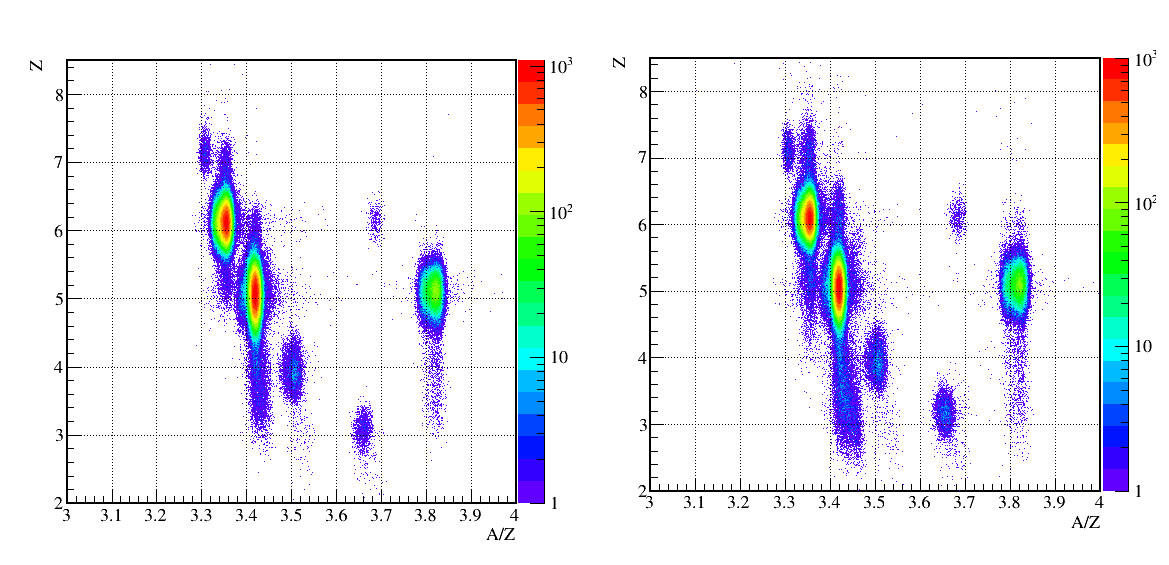
\includegraphics[width=0.8\textwidth]{chapter4/beampid.png}
    \caption[Secondary beam particle identification]{Beam particle identification of the secondary beam}
    \label{fig:Beam_PID}
\end{figure}

The gate condition for $^{17}$B is as follows.
\begin{itemize}
    \item DSB trigger 
    \item effective area of target $x <$ $\pm$ 35 mm and $y <$ $\pm$ 35 mm
    \item $4.40 < Z < 5.69$ and $3.4 < A/Z < 3.44$

\end{itemize}


\begin{table}[h]
    \centering
    \begin{tabular}{cccc}
        \hline
        Secondary Beam & Pb target & C target & Empty target\\             
        \hline
        ${}^{17}$B & 829586 & 756021 & 331445 \\
        ${}^{19}$B &  160905&  144243&  63033\\
        ${}^{20}$C &  1675080 & 1483113 & 510410 \\
        \hline
    \end{tabular}
    \caption{Statistic of secondary beam}
    \label{tab:Beam_PID}
\end{table}

%----------------------------------------------------------------------------------------------------

\section{Beam Profile at Target}

The beam profile at the target can be determined using the two drift chambers, BDC1 and BDC2, located upstream of the target. The incident position and angle at the target are obtained from the beam positions at BDC1 and BDC2.

\subsection{BDC Calibration}
The BDC drift chamber is designed for tracking the incident particle. Beam particle trajectory is obtained by following procedure.

\begin{enumerate}
    \item Obtain a drift time from TDC distribution.
    \item Extract a hit position of each layer from STC (Space to Time Conversion) function.
    \item Fit the trajectory with the linear function by the least-square method.
\end{enumerate}

\subsubsection{TDC (Time to Digital Converter) Distribution}
The timing information of the BDC is obtained by TDC (Time to Digital Converter). In figure \ref{fig:TDC_BDCs}, the TDC distribution of BDC1 and BDC2 are shown. Since we used common stop mode to take a TDC data in this experiment, the drift time is,
\begin{align}
    t_{drift} = t_{max} - t_{\text{TDC}}
\end{align}
where $t_{max}$ is the maximum TDC value. This TDC distribution is obtained from run 431 with $\pm$ 5mm slit at F5. 

\subsubsection{STC (Space to Time Conversion) Function}
The distance between hit position to an anode wire is given by space time conversion (STC) from the drift time. Assuming the uniform position distribution in each drift length cell as
\begin{align}
    \frac{dN}{dx} = const.  
\end{align}
The STC function is derived by integrating the TDC distribution as,
\begin{align}
    &\frac{dN}{dt} \cdot \frac{dt}{dx} = const.\\
    &dx = C \cdot \frac{dN}{dt} \cdot dt,\\
    &x(t) = C \cdot \int_{t_{0}}^{t} \frac{dN}{dt} dt \label{eq:stc}
\end{align}
where, C is normalization factor, $t_0$ is the minimum drift time and $t$ is the drift time from TDC distribution. 
The integration range of TDC for each BDC is shown in table \ref{tab:TDC_BDCs}. The upper and lower limit is determined by the TDC distribution. (Figure \ref{fig:TDC_BDCs}) 
\begin{table}[h]
    \centering
    \begin{tabular}{c|cc}
        \hline
        &Lower limit [ch]& Upper limit [ch]\\
        \hline
        BDC1&640&760\\
        BDC2&630&750\\        
        \hline
    \end{tabular}
    \caption[TDC integration ranges of BDCs]{TDC integration ranges of BDC1 and BDC2}
    \label{tab:TDC_BDCs}
\end{table}

\begin{figure}[h]
    \centering
    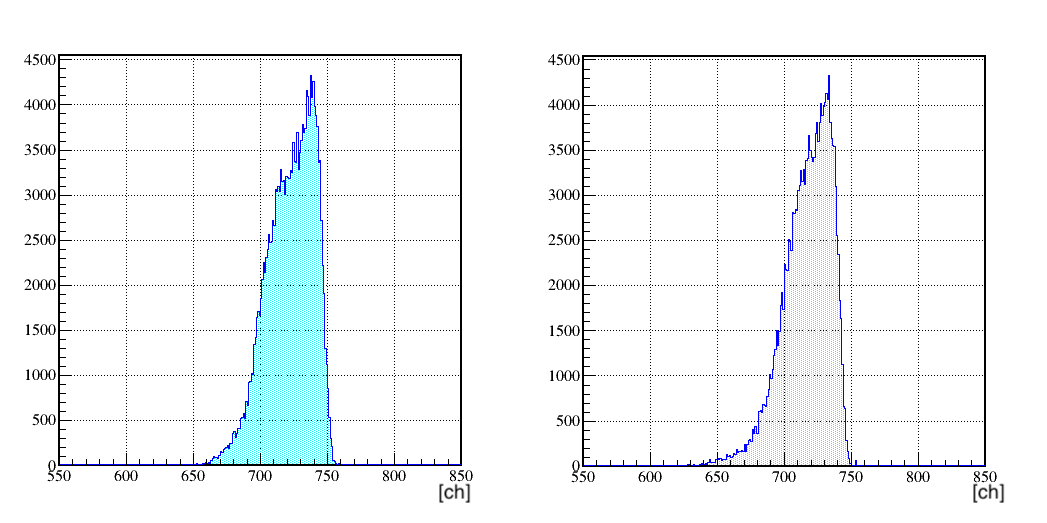
\includegraphics[width=14cm]{chapter4/BDCs_TDC.png}
    \caption[TDC Distribution of BDCs]{TDC Distribution of BDC1 (left) and BDC2 (right)}
    \label{fig:TDC_BDCs}
\end{figure}

\subsubsection{Linear fitting of trajectory}
After getting the STC function, the hit position of each layer is calculated from drift time as eq. (\ref{eq:stc}). Now we can get the trajectory of beam particle by fitting the hit position with linear function. When fitting the trajectory, the least-square method is used. The least-square method is the method of finding the best fit of a set of hit positions by minimizing the $\chi^2$ value. The $\chi^2$ value is defined as,
\begin{align}
    \chi^2 = \sum_{i=1}^{N} \frac{(x_{i} - f(x_{fit}))^2}{\sigma_{i}^2}
\end{align}
where, $x_{i}$ is the hit position of each layer, $f(x_{fit})$ is the position from fitting function, $\sigma_{i}$ is the position resolution of each layer.

\subsubsection{The resolution of BDCs}
After tracking the trajectory, the resolution of BDCs can be evaluated by the tracking residue distribution. The tracking residue $x_{residue}$ is defined as,

\begin{align}
    x_{residue} = x_{trac} - x_{drift}
\end{align}

where $x_{trac}$ is the calculated position from the trajectory and $x_{drift}$ is the hit position of each layer. The tracking residue distribution of BDC1 and BDC2 are shown in Figure \ref{fig:residue_bdcs}. The width of residue distribution for $x$ and $y$ direction are $\Delta x$ = 0.2605 mm, $\Delta y$ = 0.2632 mm respectively. From this, the position and angular resolution are calculated as described in the Appendix A. The result is described in table \ref{tab:resolution_bdcs}.

\begin{figure}
    \centering
    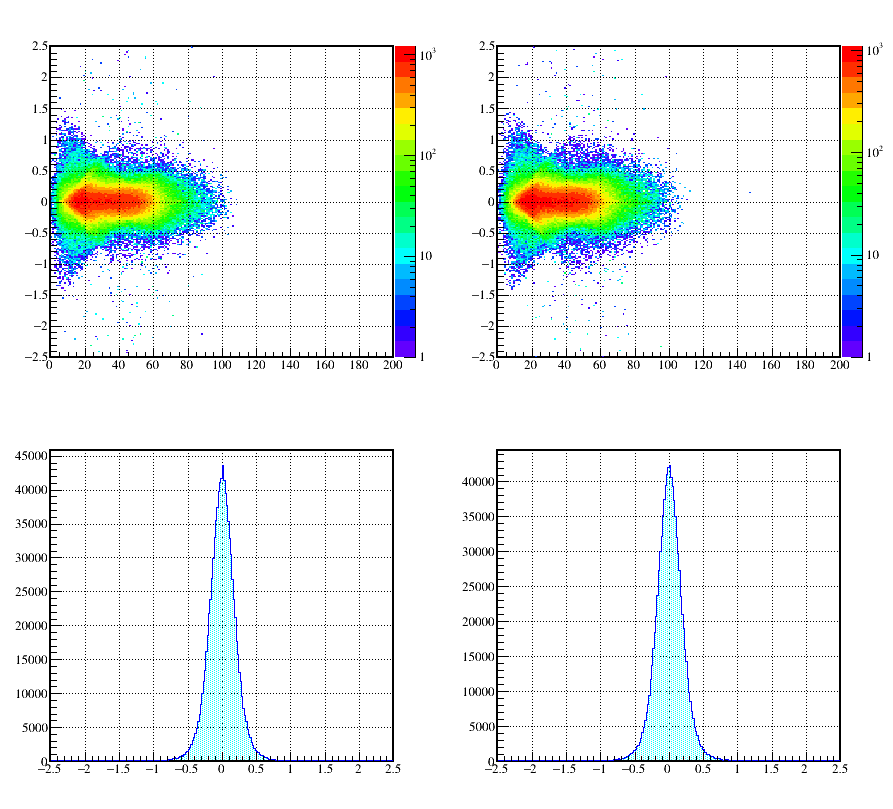
\includegraphics[width=12cm]{chapter4/BDC_residu.png}
    \caption[Tracking Residue Distribution of BDCs]{Tracking Residue Distribution of BDC1 (left) and BDC2 (right)}
    \label{fig:residue_bdcs}
\end{figure}

\begin{table}
    \centering
    \begin{tabular}{c|cc}
    \hline
     & $\sigma_x$ [mm] & $\sigma_y$ [mm]\\
    \hline
    BDC1 & 0.1340 & 0.1627 \\
    BDC2 & 0.1422 & 0.1743 \\
    \hline 
    \hline
    & $\sigma_a$ [rad] & $\sigma_b$ [rad]\\
    \hline
    BDC1 & 0.01316 & 0.01330 \\
    BDC2 & 0.01396 & 0.01424 \\
    \hline
    \end{tabular}
    \caption{Position and Angular Resolution of BDCs}
    \label{tab:resolution_bdcs}
\end{table}

\clearpage

\subsection{Beam Profile at Target}
The beam profile at the target is obtained by using the position information from BDCs. The position information ($x_{\text{tgt}}$, $y_{\text{tgt}}$) and angle information ($a_{\text{tgt}}$, $b_{\text{tgt}}$) at the target are obtained as,

\begin{align}
    x_{\text{tgt}} &= x_{\text{BDC1}} + \frac{(x_{\text{BDC2}} - x_{\text{BDC1}})}{L(\text{BDC1} - \text{BDC2})} \times L(\text{BDC1} - \text{tgt})\\
    y_{\text{tgt}} &= y_{\text{BDC1}} + \frac{(y_{\text{BDC2}} - y_{\text{BDC1}})}{L(\text{BDC1} - \text{BDC2})} \times L(\text{BDC1} - \text{tgt})\\
    a_{\text{tgt}} &= tan^{-1} \bigg( \frac{(x_{\text{BDC2}} - x_{\text{BDC1}})}{L(\text{BDC1} - \text{BDC2})} \bigg)\\
    b_{\text{tgt}} &= tan^{-1} \bigg( \frac{(y_{\text{BDC2}} - y_{\text{BDC1}})}{L(\text{BDC1} - \text{BDC2})} \bigg),
\end{align}
where the distance between BDCs is $L(\text{BDC1} - \text{BDC2}) = 999.32$mm, and the distance between BDC1 and the target is $L(\text{BDC1} - \text{tgt}) = 2017.13$mm. The beam profile at the target is shown in Figure \ref{fig:beam_profile_tgt}.
\begin{figure}[h]
    \centering
    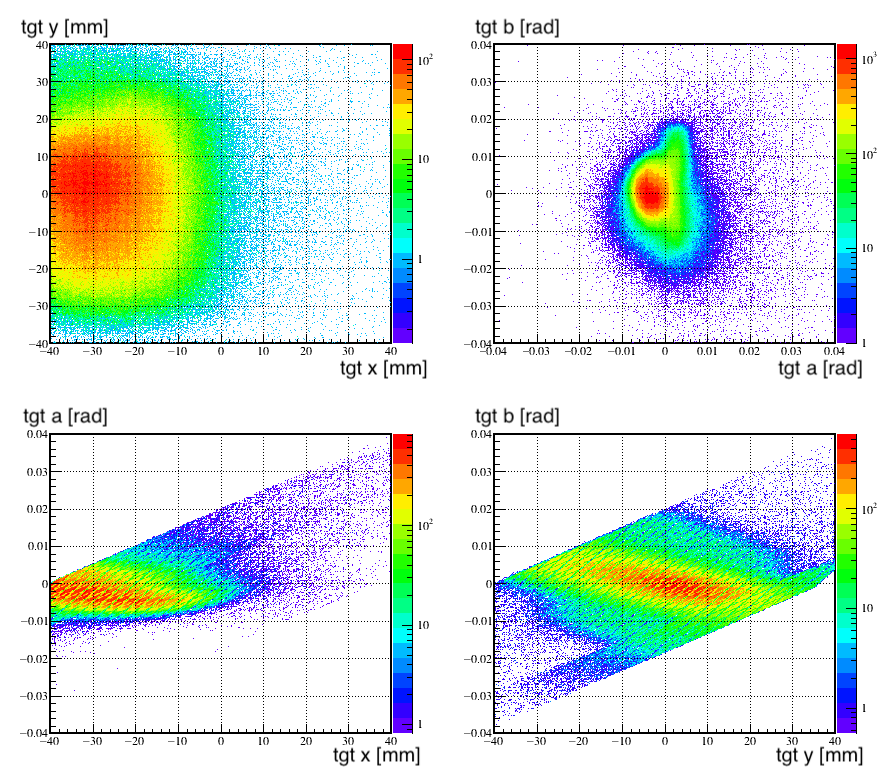
\includegraphics[width=10cm]{chapter4/target.png}
    \caption{${}^{17}$B Beam profile at target}
    \label{fig:beam_profile_tgt}
\end{figure}

\subsection{Position and Angular Resolution at Target}
\begin{align}
    \Delta \theta_x^{\text{tgt}} = \Delta \bigg( \frac{x_{\text{BDC2}} - x_{\text{BDC1}}}{L(\text{BDC2} - \text{BDC1})} \bigg) 
    = \frac{\sqrt{(\Delta x_{\text{BDC2}})^2 + (\Delta x_{\text{BDC1}})^2}}{999.32 \text{mm}} = 0.196 \text{mrad}\\
    \Delta \theta^{\text{tgt}}_y = \Delta \Big( \frac{y_{\text{BDC2}} - y_{\text{BDC1}}}{L(\text{BDC2} - \text{BDC1})} \Big) 
    = \frac{\sqrt{(\Delta y_{\text{BDC2}})^2 + (\Delta y_{\text{BDC1}})^2}}{999.32 \text{mm}} = 0.239 \text{mrad}
\end{align}
The position resolution at the target is
\begin{align}
    \Delta x_{\text{tgt}} = \sqrt{(\Delta x_{\text{BDC2}})^2 + (\Delta \theta_x^{\text{tgt}} \cdot L(\text{tgt} - \text{BDC2}))^2} = 0.24 \text{mm}\\ 
    \Delta y_{\text{tgt}} = \sqrt{(\Delta y_{\text{BDC2}})^2 + (\Delta \theta_y^{\text{tgt}} \cdot L(\text{tgt} - \text{BDC2}))^2} = 0.28 \text{mm}
\end{align}

\clearpage

\section{Charged Particle Identification}

Charged particles are identified using the TOF-B$\rho$-$\Delta$E method as same as the beam particle identification. Time of Flight is obtained from time difference between target and HODF, $B\rho$ is calculated from FDC1 and FDC2 positions and angles, and $Z$ is calculated by HOD $Q$ information. $A/Z$ and $Z$ is obtained by the following equation.

\begin{align}
    &\beta_{\text{frag}} = L(\text{tgt - HODF}) / ( {\text{TOF}}_{\text{tgt - HODF}} \times c )\\
    &A/Z = \frac{c \times B\rho \times \gamma_{\text{frag}}} { m_u \times \beta_{\text{frag}}}\\
    &Z = p_0 + p_1 (Q_{\text{HOD}} - p_2 \frac{1}{\beta^2})
\end{align}

$L$(tgt - HODF) is flight length from target to HODF. This is also calculated by a function of the positions and angles at FDC1 and FDC2 as the one for $B\rho$. The coefficient of $Z$ calculation $p_0, p_1, p_2$ are obtained by linear fitting of HOD $Q$ distribution. The detail of each steps will be described in following.

\subsection{FDC Calibration}
The tracking procedure of FDCs is same as BDC. The integration range of TDC for each FDC is shown in table \ref{tab:TDC_FDCs} And the TDC distribution for determining the upper and lower limit are shown in Figure \ref{fig:TDC_FDCs}. 
\begin{table}[h]
    \centering
    \begin{tabular}{c|cc}
        \hline
        &Lower limit [ch]&Upper limit [ch]\\
        \hline
        FDC1&1300&1600\\
        FDC2&500&1470\\        
        \hline
    \end{tabular}
    \caption[TDC integration range of FDCs]{TDC integration ranges of FDC1 and FDC2}
    \label{tab:TDC_FDCs}
\end{table}

\begin{figure}
    \centering
    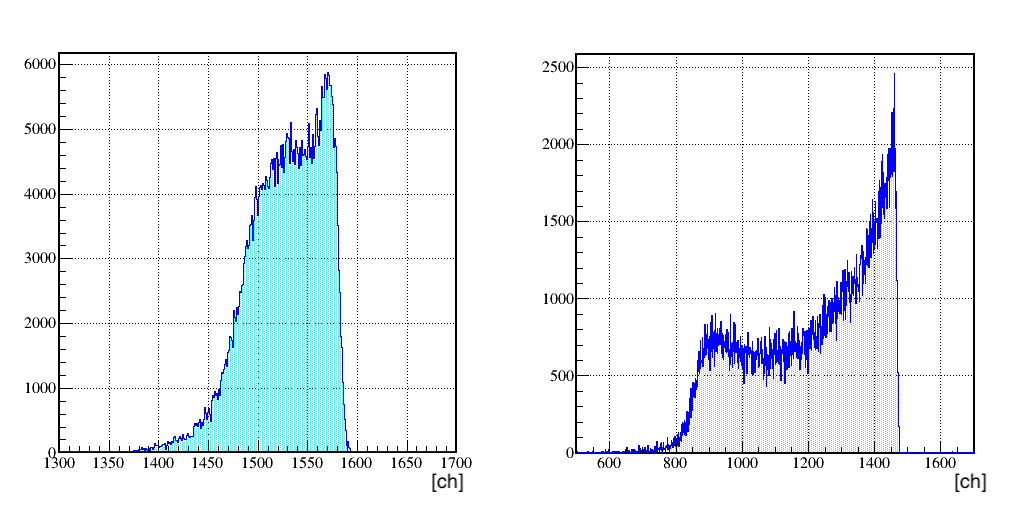
\includegraphics[width=14cm]{chapter4/FDCs_TDC.png}
    \caption[TDC Distribution of FDCs]{TDC Distribution of FDC1 (left) and FDC2 (right)}
    \label{fig:TDC_FDCs}
\end{figure}

\subsubsection{The resolution of FDCs}
The residue distributions of all plane of FDCs are shown in Figure \ref{fig:residue_fdcs}. From this, the position and angular resolution are calculated as described in the Appendix A. The result is described in table \ref{tab:resolution_fdcs}.

 \begin{figure}
    \centering
    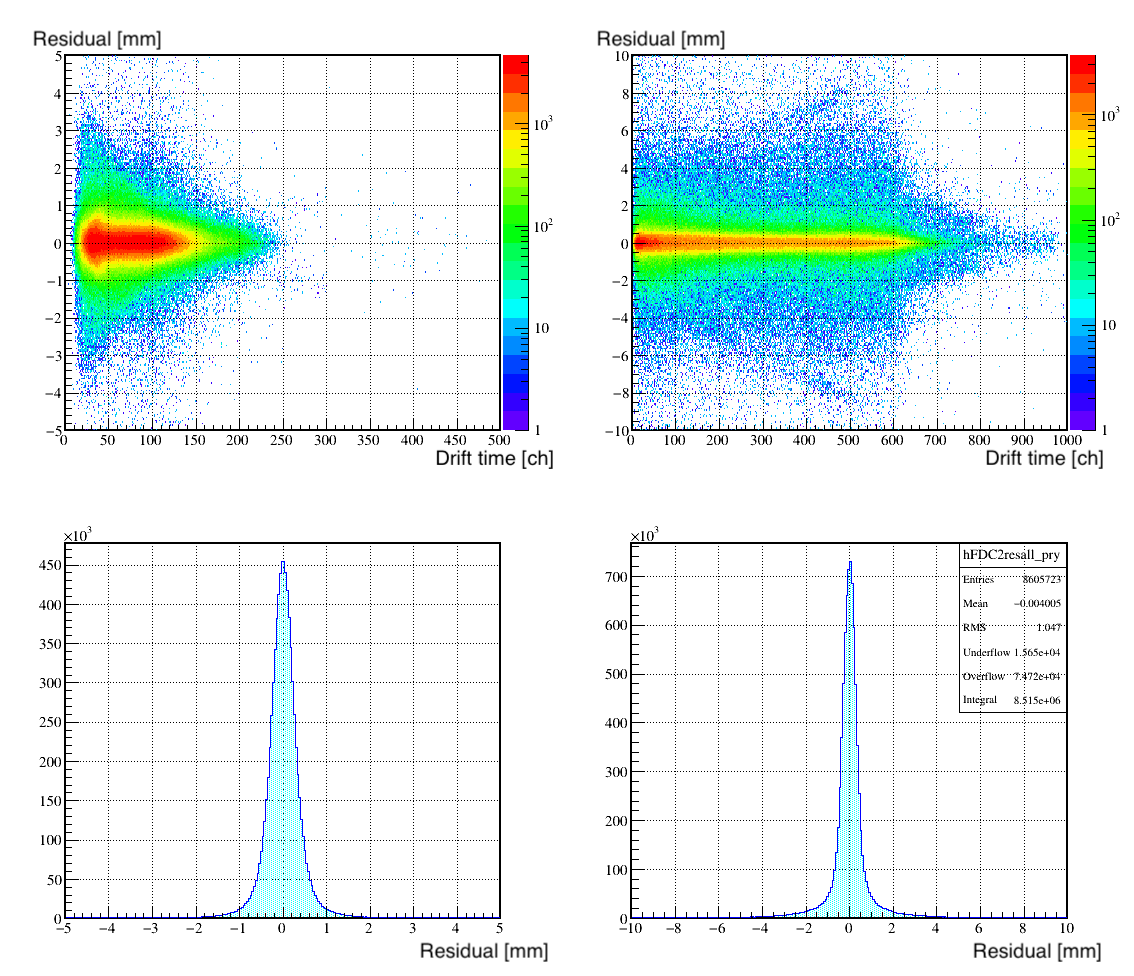
\includegraphics[width=12cm]{chapter4/FDC_residu.png}
    \caption[Tracking Residue Distribution of FDCs]{Tracking Residue Distribution of FDC1 (left) and FDC2 (right)}
    \label{fig:residue_fdcs}
\end{figure}

\begin{table}[h]
    \centering
    \begin{tabular}{c|cc}
        \hline
                &  $\Delta x_0$ [mm] & $\Delta y_0$ [mm]\\
            \hline
            FDC1 & 0.1239 & 0.2944 \\
            FDC2 &  0.1450 & 0.3443\\
            \hline
    \end{tabular}

    \begin{tabular}{c|cc}
    \hline
        & $\Delta a_0$ [rad] & $\Delta b_0$ [rad]\\
        \hline
        FDC1 & 0.00289 & 0.00948\\
        FDC2 & 0.00068 & 0.00224 \\
        \hline
    \end{tabular}
    \caption{Position and angular resolution of FDCs}
    \label{tab:resolution_fdcs}
\end{table}

\subsubsection{The efficiency of FDCs}
The efficiency of FDCs is evaluated by the tracking efficiency. The tracking efficiency is defined as the ratio of the number of events with a track at FDCs to the number of events with a hit at HODF. The definition of each efficiency can be written in following equation.
\begin{align}
\epsilon_{\text{FDC1}} = \frac{N (\text{FDC1} \cap \text{HODF})}{N (\text{HODF})}\\    
\epsilon_{\text{FDC2}} = \frac{N (\text{FDC2} \cap \text{HODF})}{N (\text{HODF})}
\end{align}
The efficiency of FDC1 and FDC2 of $^{15}$B fragment for lead target is 96.0\% and 99.9\% respectively. The efficiency of FDC1 and FDC2 for carbon target is 93.1\% and 99.9\% respectively. And the efficiency of FDC1 and FDC2 for empty target is 98.9\% and 99.9\% respectively.

\subsection{Magnetic Rigidity}
The Brho of the charged particle is calculated from the positions and angles obtained from FDC1 and FDC2. The $B\rho$ is calculated by the following equation.
\begin{align}
    B\rho &= f(x_{\text{FDC1}}, y_{\text{FDC1}}, a_{\text{FDC1}}, b_{\text{FDC1}}, x_{\text{FDC2}}, a_{\text{FDC2}})\\
    &= \sum_{i} c_{1,i} a_i + \sum_{i}\sum_{j} c_{2,ij} a_i a_j + \sum_{i}\sum_{j}\sum_{k} c_{3,ijk} a_i a_j a_k + \cdots \\
    &= c_{1,0} x_{\text{FDC1}} + c_{1,1} y_{\text{FDC1}} + \cdots + c_{2,00} x_{\text{FDC1}}^2 + c_{2,01} x_{\text{FDC1}} y_{\text{FDC1}} + \cdots + c_{3,000} x_{\text{FDC1}}^3 + \cdots
\end{align}
The function of B$\rho$ is extracted by using TMultiDimFit class in ROOT using a trajectory obtained from Geant4 simulation.

\subsection{Time of Flight and Energy Loss}
\subsubsection{Time of Flight}
Time of flight of charged particle is determined by the time difference between the HODF and the target. The time at target is determined by addition of the time at F13 and the time of flight from F13 to the target. The time of flight between F13 and the target is calculated with ${}^{17}$B beam with Energy loss calculation considered the material between F13 and the target. The time of flight between HODF and target is defined by the following equation.

\begin{align}
    t_{\text{tgt}} = t_{F13} + tof_{\text{F13-tgt}}
    tof_{\text{HODF-tgt}} = t_{\text{HODF}} - t_{\text{tgt}} + \Delta t_{offset}
\end{align}
where $t_{\text{HODF}}$ is timing information of HODF and $\Delta t_{offset}$ is obtained by Geant4 simulation as same as B$\rho$ analysis. The $\Delta t_{offset}$ is defined as 112.53 ns.

\subsubsection{Energy Loss}
In case of fragment, the energy loss is obtained from the light output information of HODF scintillator. From the Bethe-Bloch formula, we assumed that 
\begin{align}
    Z_{frag} \propto \beta_{frag} \sqrt{\Delta E} = \beta_{frag} \sqrt{Q_{\text{HODF}}}.
\end{align}
$\beta_{frag}$ is obtained from the time of flight information and $Q_{\text{HODF}}$ is the light output information of HODF. Because of the proportional relation between $Z_{frag}$ and $\sqrt{Q_{\text{HODF}}}$, it is difficult to identify the fragment particle by only energy loss information. So first we gate the fragment particle by ${}^{17}$B beam, and assumed that most of fragment came from ${}^{17}$B should be ${}^{17}$B itself. Then we can get coefficient for calculating the $Z$.

\subsection{Fragment Particle Identification}
The fragment particle identification is shown in figure \ref{fig:fragpid_all} and \ref{fig:fragpid_b17}. Figure \ref{fig:fragpid_all} is the fragment particle identification of all events. Figure \ref{fig:fragpid_b17} is the fragment particle identification only from ${}^{17}$B beam events. We selected the $^{15}$B events with $4.735 < Z < 5.275$ and $2.95 < A/Z < 3.07$ and $^{13}$B events with $4.735 < Z < 5.275$ and $2.58 < A/Z < 2.70$.
\begin{figure}
    \centering
    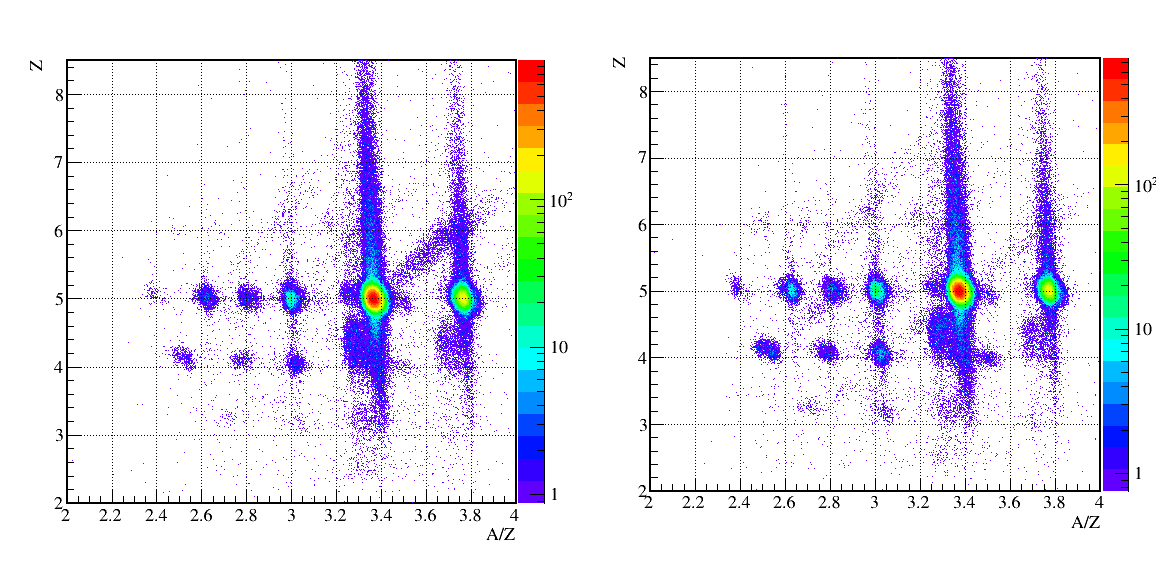
\includegraphics[width=\textwidth]{chapter4/fragpid_all.png}
    \caption[Fragment particle identification]{Fragment particle identification of all events at Pb target (left) and C target (right)}
    \label{fig:fragpid_all}
\end{figure}

\begin{figure}
    \centering
    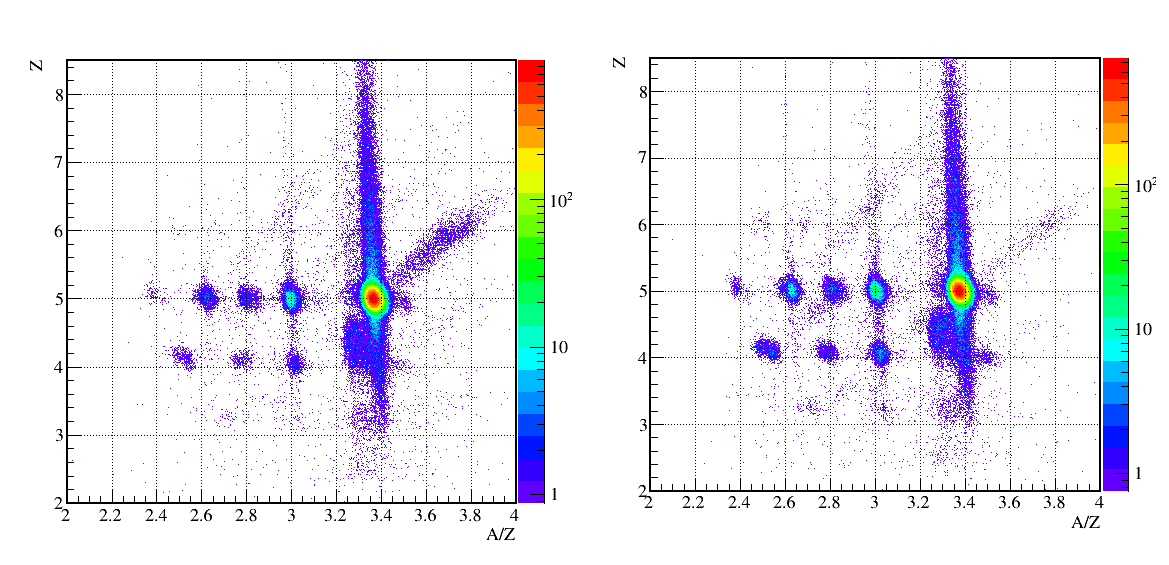
\includegraphics[width=\textwidth]{chapter4/fragpid_b17.png}
    \caption[Fragment particle identification from ${}^{17}$B beam]{Same as Figure\ref{fig:fragpid_all} but gated by ${}^{17}$B events at Pb target (left) and C target (right)}
    \label{fig:fragpid_b17}
\end{figure}

\clearpage

\section{Analysis of Neutrons}
In this experiment, neutrons emitted in the breakup reaction from the secondary beam ${}^{17}$B are detected by the NEBULA neutron detector array. A neutron is detected indirectly by recoiled proton which is mainly produced by H($n$,$n$) and ${}^{12}$C($n$,$np$) reaction in the plastic scintillator. The vector of neutron is determined as follows.
\begin{align}
    L &= | \vec{r}_{\text{tgt}} - \vec{r}_{n} | \\
    \beta_{n} &= L / (\text{TOF}_{\text{NEB-tgt}} \times c) \\
    P_{n} &= m_{n} \beta_{n} \gamma_{n} \\
    E_{n} &= m_{n} \gamma_{n} \\
    \vec{P_{n}} &= \frac{\vec{r_{n}} - \vec{r_{tgt}}}{L} P_{n}
\end{align}
where, $\vec{r}_{\text{tgt}}$ is the position of the target $\vec{r}_{\text{tgt}}$, $m_{n}$ is the neutron mass. In following section, the analysis of neutron events will be described.

\subsection {Selection of Real Neutron Events}
For the selection of neutron events, the events caused by charged particle and gamma ray should be rejected. In addition, in two neutron selection procedure, noise signals caused by multiple interaction of a single neutron, called cross-talk have to be eliminated. The selection of neutron events is performed in five steps as follows. 
\begin{enumerate}
    \item All events detected by the first VETO are considered to be charged particles and are rejected.
    \item Among the events detected by NEBULA, events with a light output Q of less than 6 MeVee are considered to be gamma rays and are rejected.
    \item Events whose TOF from the target to the first wall is less than 40 ns and whose TOF from the target to the second wall is less than 42 ns are considered to be non-neutron events with $\beta < 0.9$ and are rejected.
    \item (For the selection of two neutron events) For events detected at the second VETO, detections in which the two fastest neutron events incident on the second NEUT wall are dr(xy) $<$ 500mm and 1ns $<$ dt $<$ 5ns are considered to be cluster scattering events from second VETO and the second event is rejected.
    \item (For the selection of two neutron events) Cross-talk events are rejected.
\end{enumerate}
After these rejection procedure, we choose the first and second fastest event as a neutron event. In following section, the three step of cross-talk rejection procedure will be described.

\subsection{Cross-talk Rejection}
The conditions of the cross-talk rejection are determined based on a Geant4 simulation. To reject the cross-talk events, ${}^{16}\text{B} \to {}^{15}\text{B}+n$ simulation is performed, thereby replicating cases where all two-neutron events are due to cross-talk. The beam $^{16}$B is reconstructed based on the $^{17}$B beam information at target (Figure \ref{fig:beam_profile_tgt}). The details of the simulation are shown in Table \ref{tab:cross-talk_sim}.

\begin{table}
    \centering
    \begin{tabular}[h]{c|c}
        \hline 
        Reaction & ${}^{16}\text{B} \to {}^{15}\text{B}+n$ \\
        Beam energy & Reconstructed from $^{17}$B beam profile\\
        Relative energy & 0 - 10 MeV (Uniformly generated)\\
        Position distribution & Reconstructed from ${}^{17}$B beam profile\\
        Angular distribution & Reconstructed from ${}^{17}$B beam profile \\
        \hline
    \end{tabular}
    \caption{The Geant4 simulation condition for cross-talk rejection}
    \label{tab:cross-talk_sim}
\end{table}

\subsubsection{Clustering event}
The clustering event means the two events which are detected in very close distance in very small time interval. It means the second event is likely to be a recoil proton from the first event. The clustering event is rejected by the following condition.

\begin{figure}[h]
    \centering
    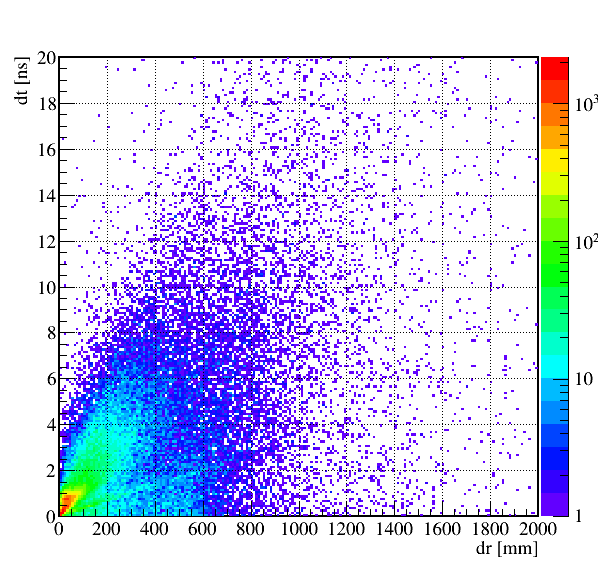
\includegraphics[width=8cm]{chapter4/drdt.png}
    \caption{Cross-talk simulation result of clustering event}
    \label{fig:clustering}
\end{figure}

\begin{align}
    \bigg( \frac{dr-dr_0}{3\sigma_{dr}} \bigg)^2 + \bigg( \frac{dt-dt_0}{3\sigma_{dt}} \bigg)^2 < 1 
\end{align}
where $dr$ and $dt$ are the position and time difference between two events. And $dr_0$ and $dt_0$, $\sigma_{dr}$ and $\sigma_{dt}$ mean the central values and the standard deviations of the distribution of $dr$ and $dt$ for the clustering events. The $dr_0$ and $dt_0$ are 98.35 mm and 0.65 ns, and $\sigma_{dr}$ and $\sigma_{dt}$ are 71.07 mm and 0.40 ns. 

\subsubsection{same wall event}
Figure\ref{fig:samewall} shows the cross-talk simulation result of same wall event. The right figure shows the distribution of light output of second event $Q_2$ with the function of relative velocity $\beta_{01}/\beta_{12}$ and the left one shows the distribution of $Q_2$ with $1/\beta_{12}$. After the selection of two neutron events, each event is tagged by the hit order. The light output is tagged as $Q_1$ and the one of second event is tagged as $Q_2$. The relative velocity between two events is defined as $\beta_{01}/\beta_{12}$ where $\beta_{01}$ represents the velocity between first hit and the target and $\beta_{12}$ represents the velocity between first and second hit. The cross-talk rejection condition of same wall event is defined as follows.
\begin{align}
    \frac{\beta_{01}}{\beta_{12}} > 1 \qquad \text{or} \qquad  \frac{\beta_{01}}{\beta_{12}} < -1.5
\end{align}

If the $\beta_{01}/\beta_{12}$ $>$ 1, it means the second event is slower than the first event and it is considered to be a cross-talk event caused by the scattered neutron from the first event. If the $\beta_{01}/\beta_{12}$ $<$ 0, it means the $z$ position of the second event is smaller than the first event. In this case, the cross-talk event can happen by the back scattering of the neutron from the first event. The condition of $\beta_{01}/\beta_{12}$ $<$ -1.5 is enough to reject this cross-talk event.
Another cross-talk rejection condition is determined by the $\gamma$ ray rejection. Considering that the $\gamma$ ray events distribute in the region of $1/\beta_{12} \sim \pm1$, the $\gamma$ ray rejection condition is defined as follows.
\begin{align}
    \bigg|\frac{1}{|\beta_{12}|} - 1\bigg| < 3\sigma_\gamma
\end{align}
The events in this region with the light output of second event $Q_2$ less than 20 MeVee are considered to be $\gamma$ ray events. The $\sigma_\gamma$ is the standard deviation of the distribution of $1/|\beta_{12}|$ for the $\gamma$ ray events. The $\sigma_\gamma$ is 0.1. 
\begin{figure}[h]
    \centering
    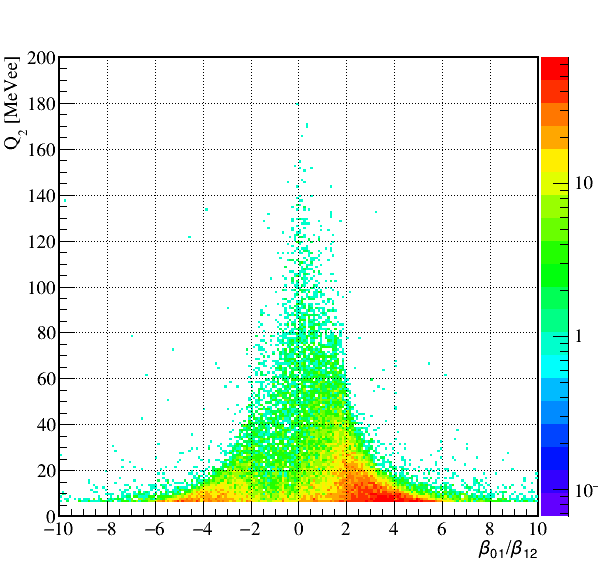
\includegraphics[width=0.4\textwidth]{chapter4/same1.png}\hspace{0.5cm}
    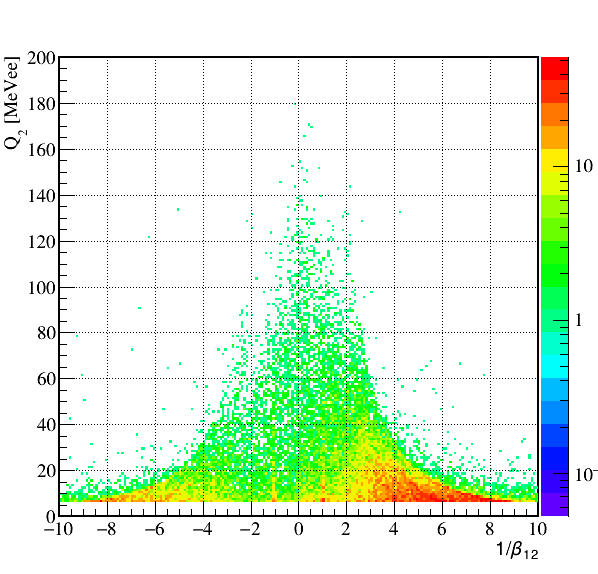
\includegraphics[width=0.4\textwidth]{chapter4/same2.png}
    \caption{Cross-talk simulation result of same wall event}
    \label{fig:samewall}
\end{figure}

\subsubsection{different wall event}
Figure \ref{fig:differentwall} shows the cross-talk simulation result of different wall event. The right figure shows the distribution of light output of second event $Q_1$ with the function of relative velocity $\beta_{01}/\beta_{12}$ and the left one shows the distribution of $Q_2$ with $1/\beta_{12}$. The cross-talk rejection condition of different wall event is similar to the same wall event, but in this case, $Q_1$ is used for the cross-talk rejection with the relative velocity. The cross-talk rejection condition of different wall event is defined as follows. 
\begin{align}
    \frac{\beta_{01}}{\beta_{12}} > 1 \qquad \text{or} \qquad  \frac{\beta_{01}}{\beta_{12}} < -1.5
\end{align}
And the $\gamma$ ray rejection is also performed using the distribution of $Q_2$ with $1/\beta_{12}$. The rejection condition is also defined as follows.
\begin{align}
    \bigg|\frac{1}{|\beta_{12}|} - 1\bigg| < 3\sigma_\gamma
\end{align}
The $\sigma_\gamma$ for different wall is 0.1.

\begin{figure}
    \centering
    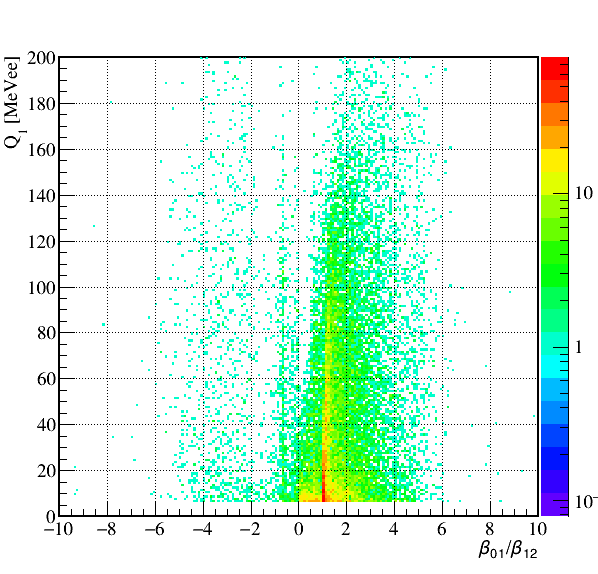
\includegraphics[width=0.4\textwidth]{chapter4/diff1.png}\hspace{0.5cm}
    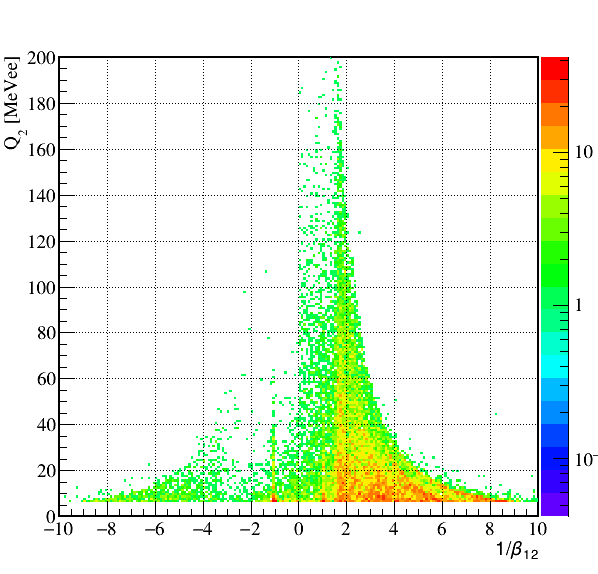
\includegraphics[width=0.4\textwidth]{chapter4/diff2.png}
    \caption{Cross-talk simulation result for different wall event}
    \label{fig:differentwall}
\end{figure}

\subsection{Cross-talk Residual Rate}
Even though we performed the cross talk rejection, there probably be residual of cross talk. For each cross talk step, we evaluated the residual rate of cross talk. Each step is as follows.
\begin{itemize}
    \item (a) no rejection
    \item (b) clustering rejection
    \item (c) clustering rejection + same wall rejection
    \item (d) clustering rejection + same wall rejection + gamma rejection
\end{itemize}
The residual rate of cross talk is given by the following equation.
\begin{align}
    R = \frac{N_{M>2}}{N_{M>1}}
\end{align}
The multiplicity $M>1$ event is 225385, $M>2$ event of each step and residual rate $R$ are written in Table \ref{cross-talk_residue}. The residual rates of same and different wall cross-talk are 2.4$\%$ and 0.9$\%$ respectively, when the all cross-talk rejection conditions are performed.
\begin{table}[h]
    \centering
    \begin{tabular}[h]{c|c|c|c}
        \hline
        Condition & same wall event (R) & different wall event (R) & all wall event (R)\\
        \hline
        (a) & 89721 (39.8$\%$) & 10123 (4.5$\%$) & 99844 (44.3$\%$) \\
        (b) & 29032 (12.9$\%$) & 16848 (7.5$\%$) & 45880 (20.4$\%$)\\
        (c) & 6274 (2.8)$\%$) & 2791 (1.2$\%$)& 9065 (4.0$\%$)\\
        (d) & 5352 (2.4$\%$)& 2089 (0.9$\%$)& 7441 (3.3$\%$)\\
        \hline
    \end{tabular}
    \caption{The cross talk residual rate evaluation}
    \label{cross-talk_residue}
\end{table}

\section{Acceptance and Efficiency Correction}
For evaluating the two-neutron detection efficiency and acceptance, the simulation is performed by Geant4. The information of simulation is as follows. The recoil effect at the reaction point is not considered in the simulation. The simulation condition is in the Table \ref{tab:2n_sim}.
\begin{table}[h]
    \centering
    \begin{tabular}[h]{c|c}
        \hline
        Physics Model & Phase Space Decay \\
        Reaction & ${}^{17}\text{B} \to {}^{15}\text{B} + 2n$\\
        Beam Energy & Reconstructed from $^{17}$B beam profile\\
        Relative Energy & 1-10 MeV (Uniformly generated)\\
        Scattering Angle & 0-30 mrad (Uniformly generated)\\
        \hline
    \end{tabular}
    \caption{The Geant4 simulation condition for two-neutron detection efficiency and acceptance}
    \label{tab:2n_sim}
\end{table}

The results of acceptance simulation for same and different wall are shown in figure \ref{fig:acc_same_diff}. $x$ axis is relative energy $E_{rel}$ between $^{15}$B and two neutrons, $y$ axis is scattering angle $\theta_{scat}$ in laboratory coordinate and $z$ axis is the detection efficiency. The acceptance of same wall in small $E_{rel}$ less than 0.5 MeV is very small because of the clustering cross-talk cut. The result of two-neutron detection efficiency curve for relative energy $E_{rel}$ is shown in figure \ref{fig:eff}. The blue line shows the same wall efficiency and the red line shows the different wall efficiency. The black line is the sum of the same and different wall efficiency. 
\begin{figure}[h]
    \centering
    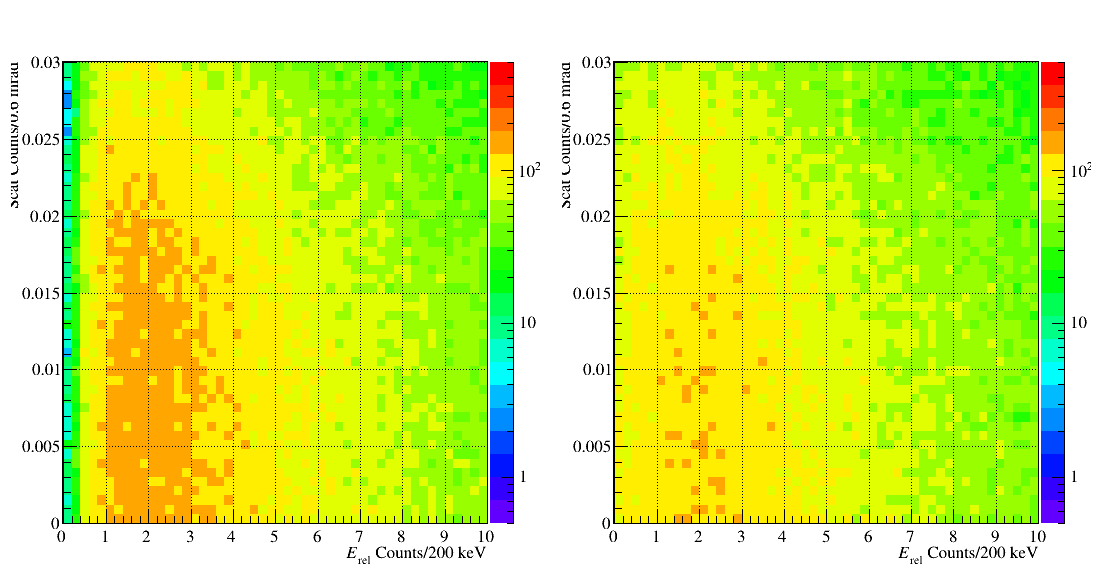
\includegraphics[width=\textwidth]{chapter4/acc_same_diff.png}
    \caption[$2n$ Acceptance for $E_{rel}$ and $\theta_{scat}$]{$2n$ Acceptance for same wall (left) and different wall (right)}
    \label{fig:acc_same_diff}
\end{figure}

\begin{figure}
    \centering
    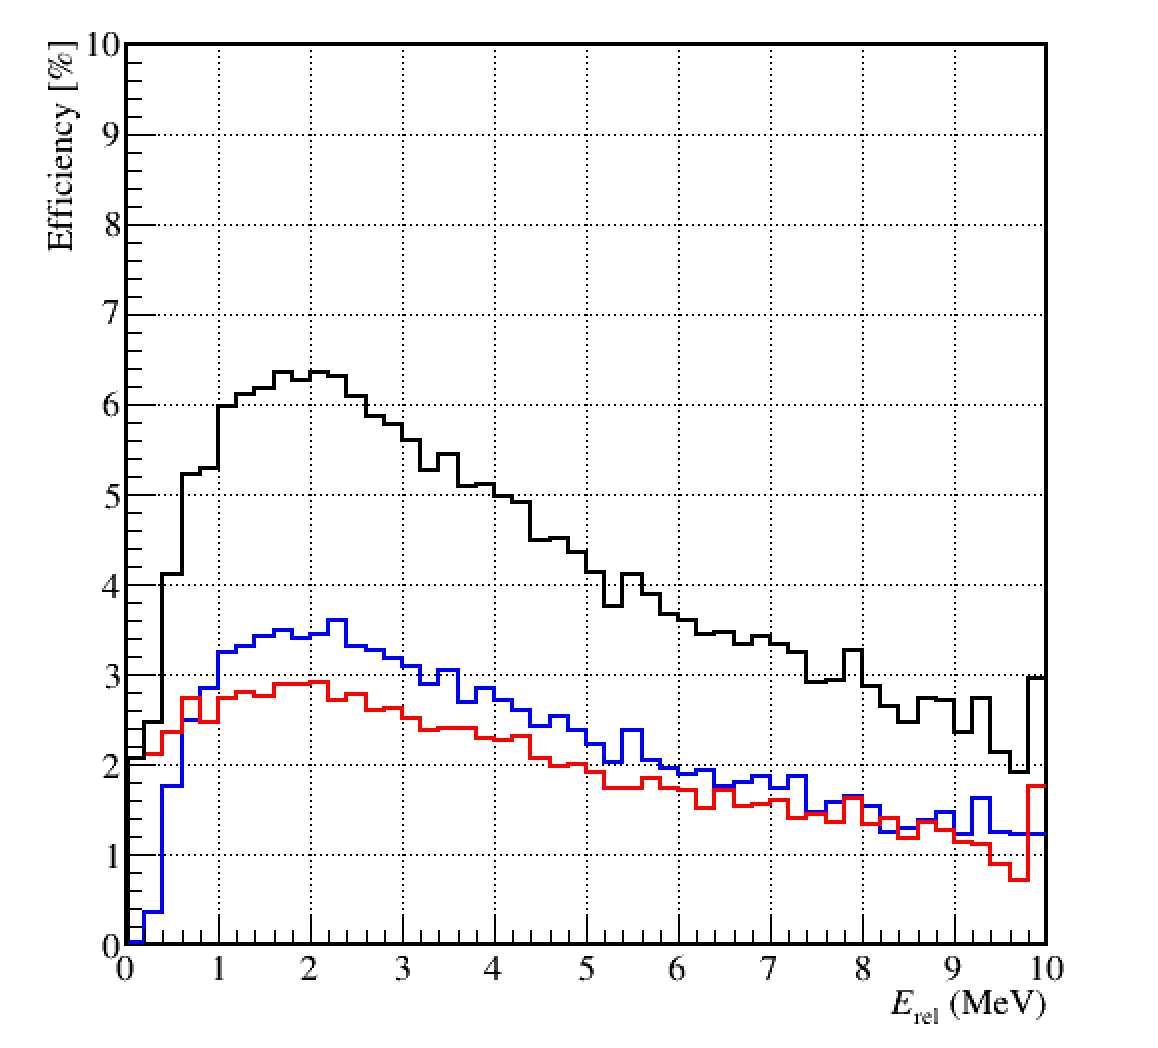
\includegraphics[width=10cm]{chapter4/Eff_curve.png}
    \caption[$2n$ detection efficiency for same wall and diff wall]{$2n$ Efficiency for same wall (left) and different wall (right)}
    \label{fig:eff}
\end{figure}

\clearpage
\section{Relative Energy Spectrum}
The relative energy $E_{rel}$ spectrum are reconstructed for the events where $^{15}$B and neutron(s) are detected. Figure \ref{fig:rel_energy_fnn} shows the relative energy spectrum of $^{15}$B and two neutrons. The relative energy spectrum of $^{15}$B and one neutron is shown in Figure \ref{fig:rel_energy_fn}. In the figures, the blue lines are the relative energy from the Pb or C target runs and the red lines are the one from empty target which is normalized with the number of events. The empty target runs will be subtracted as a background component. 
The differential cross section is calculated from the relative energy spectrum as follows.
\begin{align}
    \frac{d\sigma}{dE_{rel}} = \frac{1}{N_t} \cdot \frac{N_{i}}{N_{beam}} \cdot \frac{\text{LT}(\text{DSB})}{\text{LT}(\text{B} \cap \text{N})} \frac{1}{\epsilon_{\text{FDC1}} \epsilon_{\text{FDC2}} \epsilon_{acc} \epsilon_{eff}},
\end{align}
where $N_t$ is the number of target nucleons, $N_{i}$ is the number of events in the $i$-th bin, $N_{beam}$ is the number of beam particles, $\text{LT}(\text{DSB})$ and $\text{LT}(\text{B} \cap \text{N})$ are the live time of DSB and B $\cap$ N trigger respectively, $\epsilon_{\text{FDC1}}$ and $\epsilon_{\text{FDC2}}$ are the efficiency of FDC1 and FDC2, $\epsilon_{acc}$ is the acceptance and $\epsilon_{eff}$ is the efficiency of two-neutron detection. The differential cross section of $^{15}$B and two neutrons and $^{15}$B and one neutron are shown in Figure \ref{fig:sigma_fnn} and \ref{fig:sigma_fn}. 

\clearpage
\begin{figure}
    \centering
    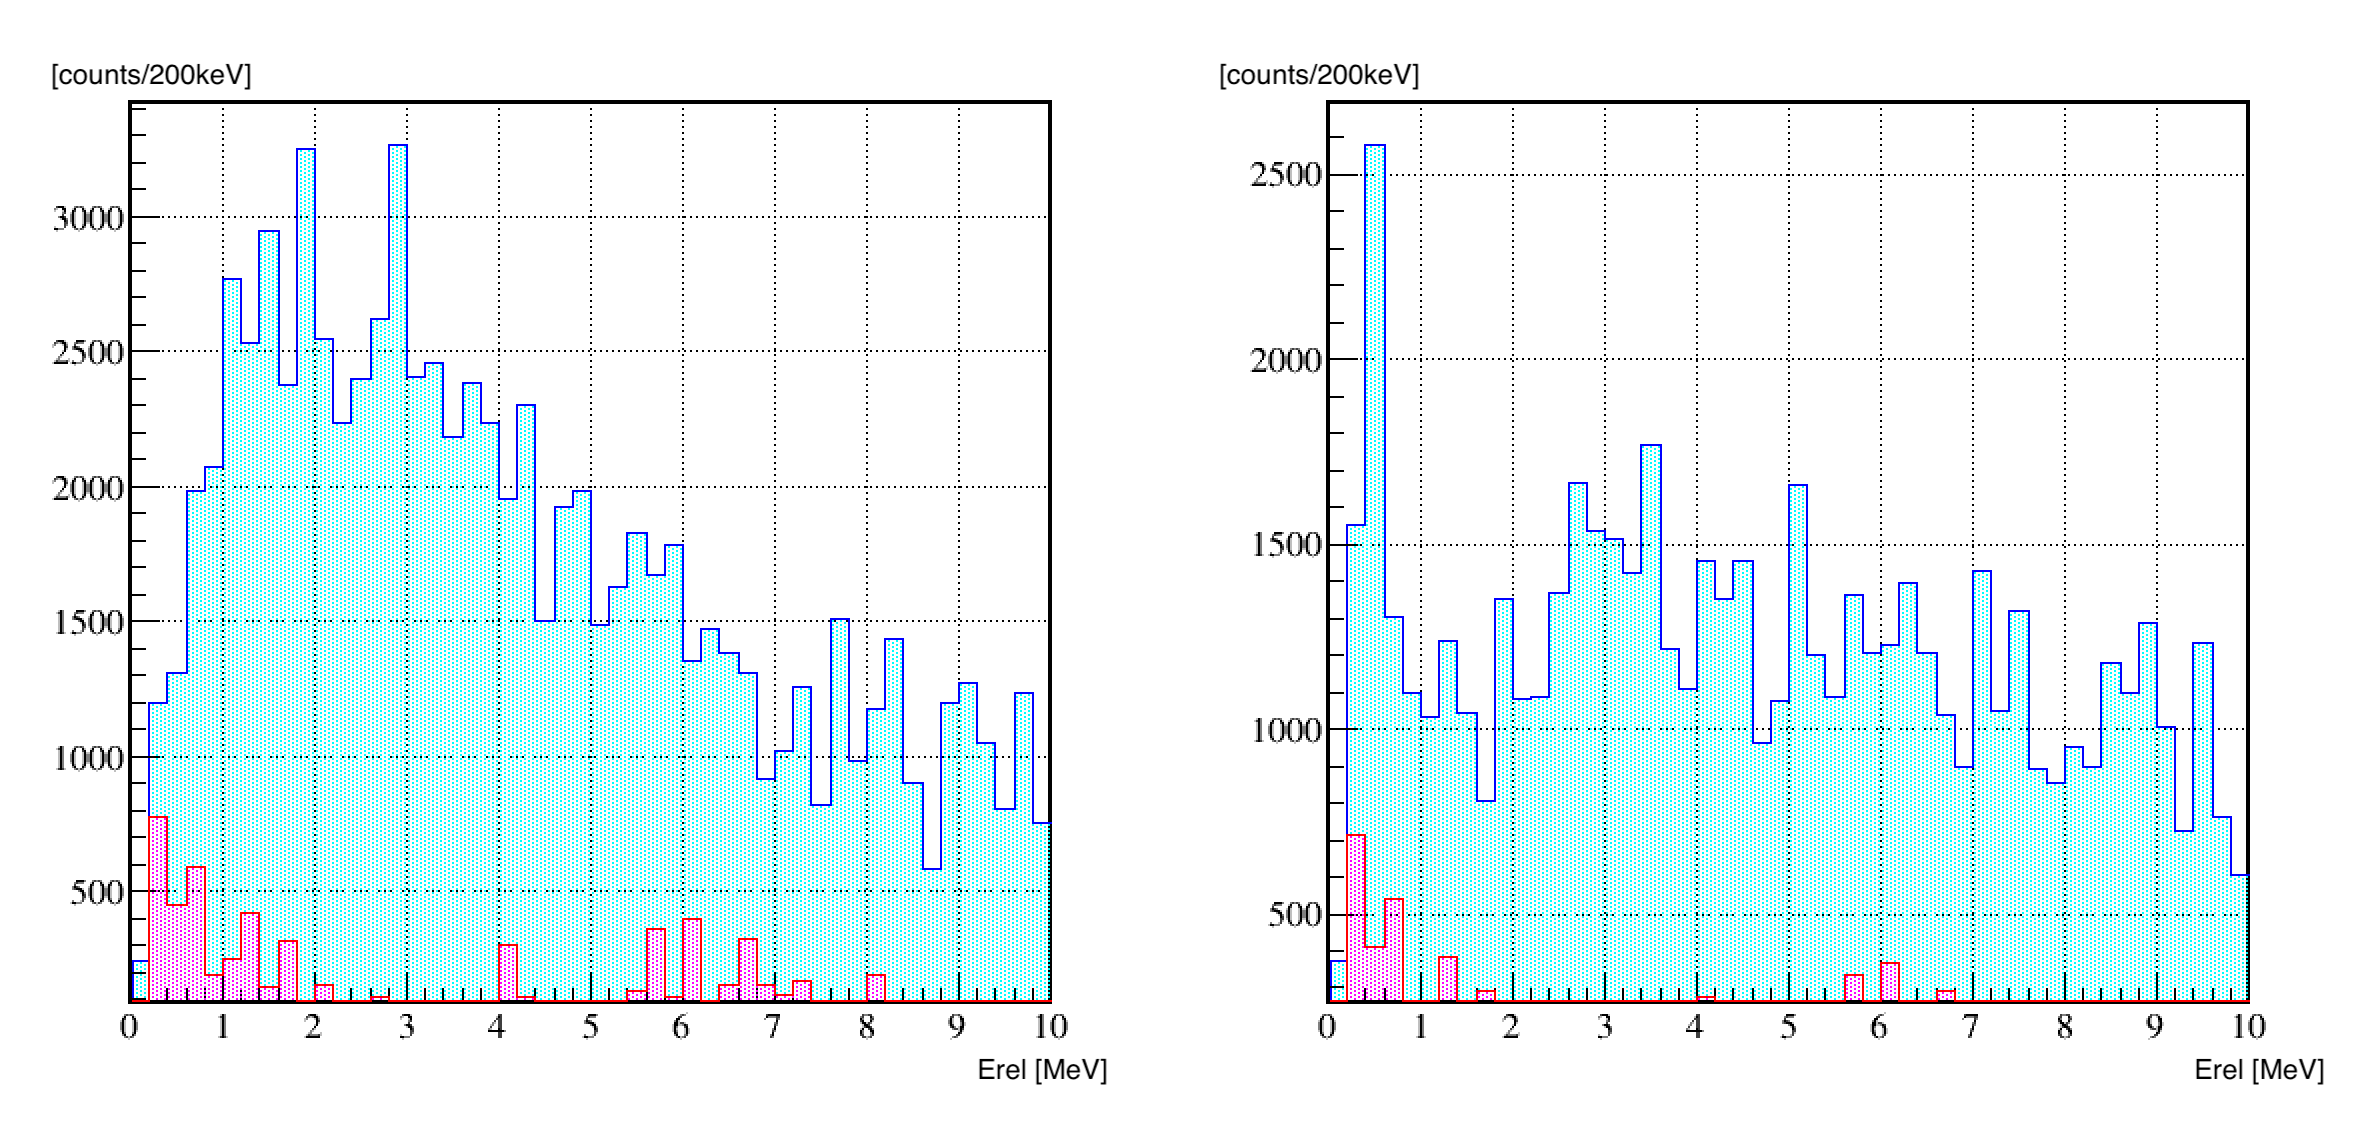
\includegraphics[width=\textwidth]{chapter4/fnn.png}
    \caption{Relative Energy Spectrum of ${}^{15}\text{B} + n + n$ at Pb target (left) and C target (right)}
    \label{fig:rel_energy_fnn}
\end{figure}

\begin{figure}
    \centering
    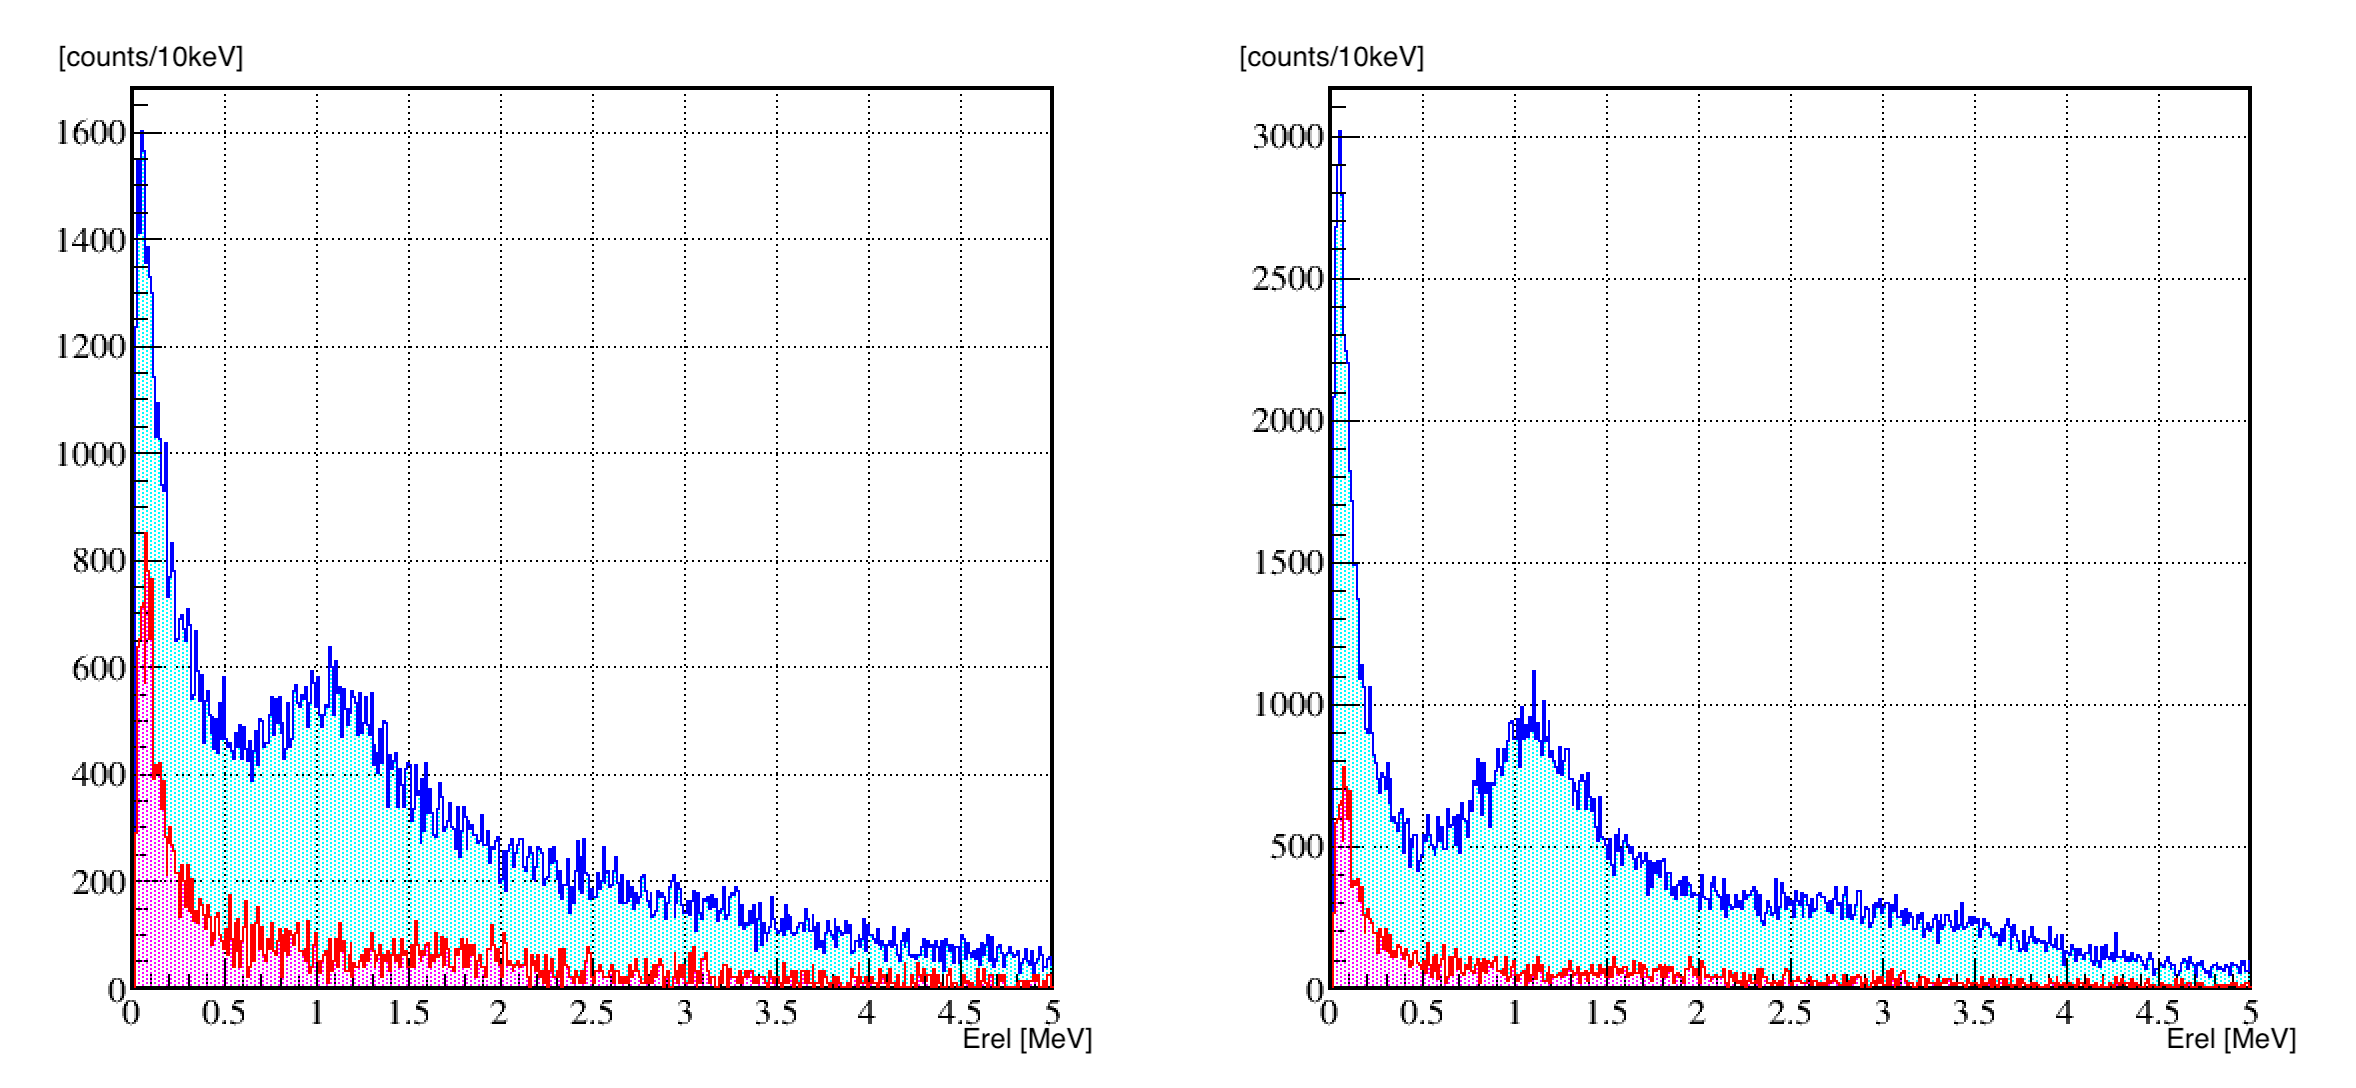
\includegraphics[width=\textwidth]{chapter4/fn.png}
    \caption{Relative Energy Spectrum of ${}^{15}\text{B} + n$ at Pb target (left) and C target (right)}
    \label{fig:rel_energy_fn}
\end{figure}

\clearpage
\begin{figure}
    \centering
    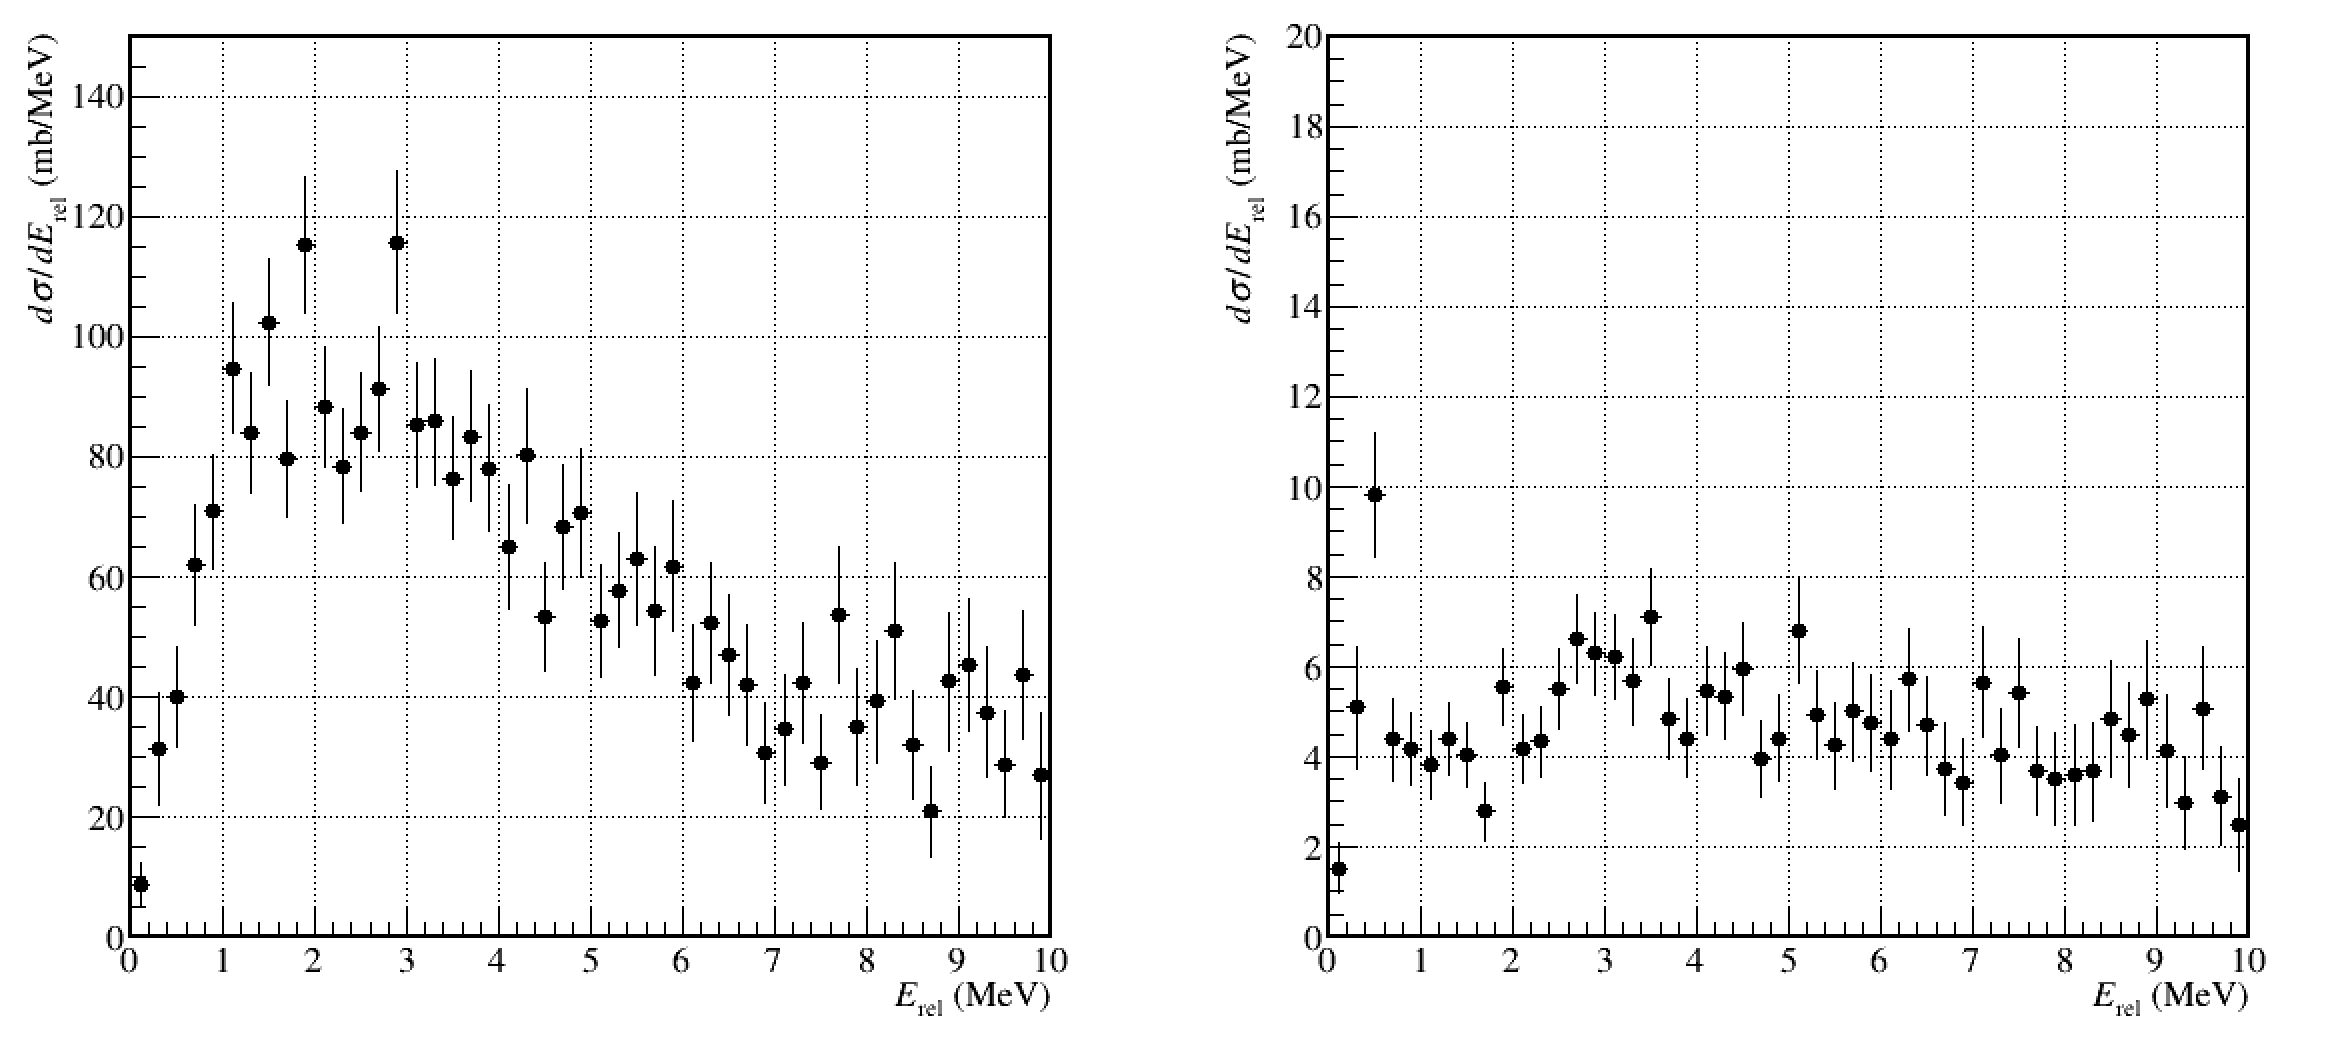
\includegraphics[width=\textwidth]{chapter4/sigma_fnn.png}
    \caption{Differential cross section of ${}^{15}\text{B} + n + n$ for Pb target (left) and C target (right)}
    \label{fig:sigma_fnn}
\end{figure}
\begin{figure}
    \centering
    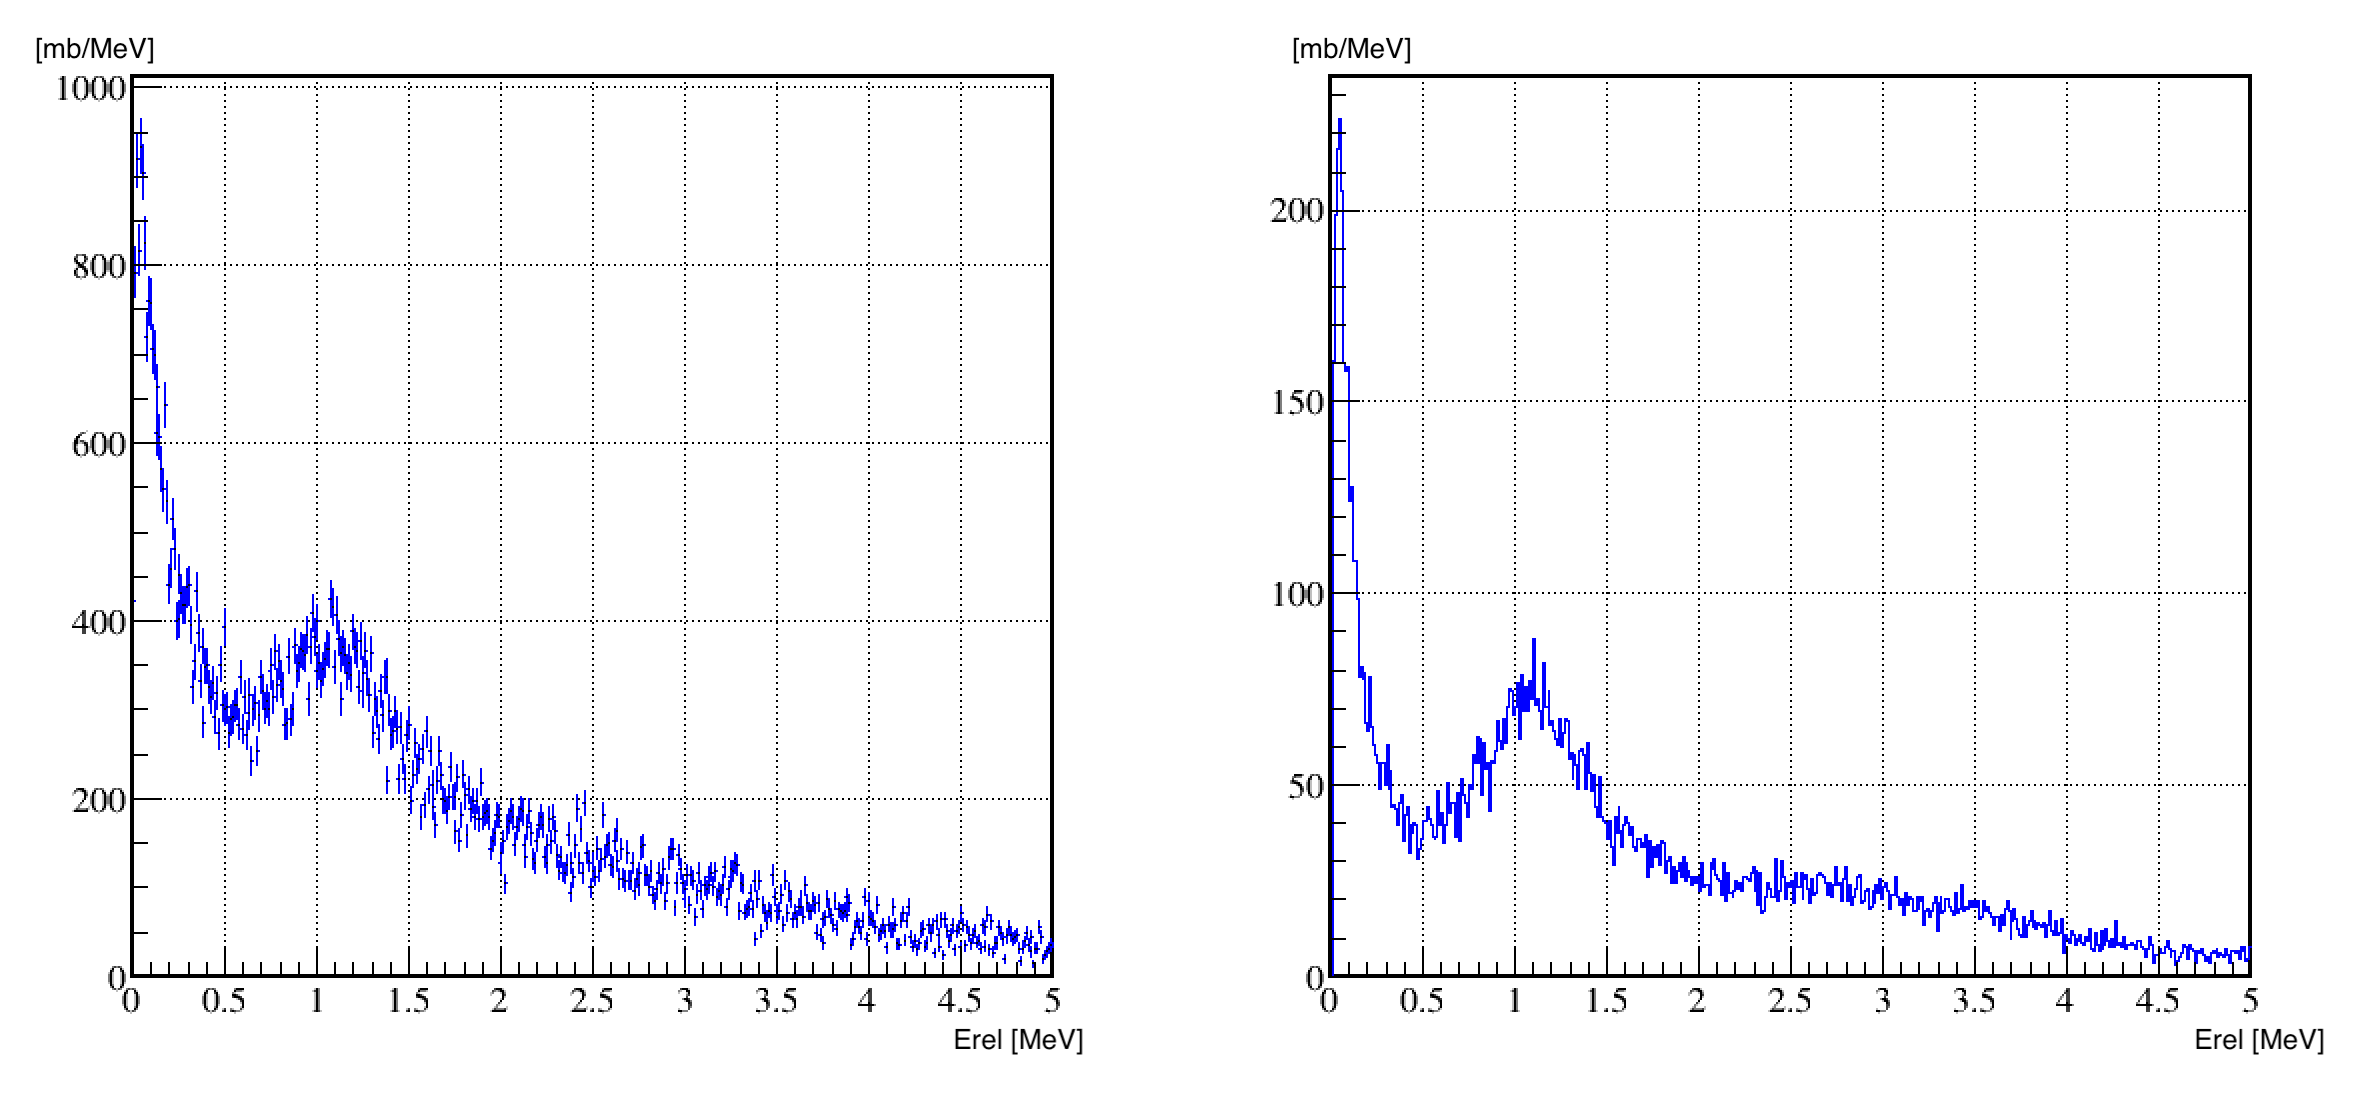
\includegraphics[width=\textwidth]{chapter4/sigma_fn.png}
    \caption{Differential cross section of ${}^{15}\text{B} + n$ at Pb target (left) and C target (right)}
    \label{fig:sigma_fn}
\end{figure}

\chapter{Result and Discussion}
xxx
\chapter{Conclusion}
In this thesis, we investigated the Coulomb dissociation of two neutron halo nucleus ${}^{17}$B with carbon and lead target at 270 MeV/u. We extracted the inclusive reaction cross section for two and four neutron removal reaction respectively. According to the 2$n$ removal reaction cross section ratio between lead and carbon target, which is 3.9, the Coulomb dissociation of $^{17}$B at lead target is not to be dominant as the neighboring nucleus $^{19}$B which has a large 2$n$ removal reaction cross section ratio, 7.1\cite{KJCook}. And the Coulomb dissociation cross section is also extracted from relative energy $E_{rel}$ spectrum. The Coulomb dissociation cross section spectrum of $^{17}$ has a broad peak around 2 $\sim$ 3 MeV, which is larger than the one of other halo nuclei such as ${}^{11}$Li\cite{Nakamura06} and $^{19}$B\cite{KJCook}. The peak position of the Coulomb dissociation cross section spectrum is related with the strength of soft $E1$ excitation of halo nuclei, and the broad peak of $^{17}$B is considered to be caused by a weak halo or a neutron skin structure. Also, by integrating the spectrum, the Coulomb dissociation cross section is obtained as 362 $\pm$ 11 mb in a range up to 7 MeV and 438 $\pm$ 13 mb up to 10 MeV. Both are significantly smaller than the one of ${}^{19}$B which is approximately 1 b\cite{KJCook}.\\
By equivalent photon method, we extracted the reduced $E1$ transition probability $B(E1)$ spectrum. The integrated $B(E1)$ value up to 7 MeV was 1.32 $\pm$ 0.06 e$^2$fm$^2$ and the one up to 10 MeV was 2.00 $\pm$ 0.10 e$^2$fm$^2$. The $B(E1)$ value for $^{19}$B was 1.64 $\pm$ 0.06 (\textit{stat}) e$^2$fm$^2$ in a range up to 6 MeV\cite{KJCook} which is larger than the one for $^{17}$B. Also, compared to the shape of $B(E1)$ spectrum for $^{19}$B, the $B(E1)$ spectrum for $^{17}$B has very broad curve and the peak position is around 4 $\sim$ 5 MeV. These features indicate that the Coulomb dissociation is not dominant for $^{17}$B as well as in the case of $^{19}$B. \\
Dineutron correlation is also investigated by the opening angle of valance neutrons. The opening angle of valance neutrons in $^{17}$B was 56.6 $\pm$ 19.4 degree in a range of $B(E1)$ up to 10 MeV, and 87.0 $\pm$ 16.6 degree in a range of $B(E1)$ up to 7 MeV. The average result has consistent with the recent research result, 77.4 degree by A. Corsi\cite{Corsi}. \\
For the future plan, evaluation of systematical error is needed. Also the contribution of excited state of $^{17}$B at the reaction point should be considered by $\gamma$ ray analysis. Also the opening angle of valance neutrons and the dineutron correlation can be calculated with a three-body model can be a theoretical support. 
\appendix
\chapter{Equations}
\section{Bethe-Bloch Formula}
Energy loss calculation for 

\section{Equivalent Photon Method}
considering multi-polarity, 
\begin{displaymath}
    n_{\pi l}(\omega)=Z^{2}_{1} \alpha \frac{l[(2l+1)]!!^{2}}{(2\pi)^{3}(l+1)}\sum_{m}\Big|G_{\pi l m}\big( \frac{c}{v}\big) \Big|^{2} g_{m}(\xi)
\end{displaymath} 

equivalent photon number for E1 excited projectile.
\begin{displaymath}
    n_{E1}(\omega)=n_{E1, m=-1}+n_{E1, m=0}+n_{E1, m=+1}=\frac{2}{\pi}Z^{2}_{1}\alpha\Big(\frac{c}{v}\Big)^{2}\Big[\xi K_{0}(\xi)K_{1}(\xi)-\frac{v^{2}\xi^{2}}{2c^{2}}(K^{2}_{1}(\xi)-K^{2}_{0}(\xi)\Big]
\end{displaymath}

with 
\begin{align}
    \xi=E_{\gamma}R/\gamma \nu \hbar\\
    E_{\gamma}: Photon energy( E_{\gamma}=\omega\hbar )\\
    Z_{1}: Atomic number of target
\end{align}
R: impact parameter ( 1.3 )\\


\chapter{Appendix B}
\section{Resolution Evaluation}

\begin{table}[h]
    \centering
    \begin{tabular}[h]{c|c}
        \hline
        Flight length & Distance \\
        \hline
        F7-F13 & 7.5m \\
        dist-BDC1-BDC2 & 1.5m \\
        dist-BDC1-tgt & 1.5m \\
        target z & 0.5m \\
        dist-FDC1-Tgt & 1.5m \\
        dist-FDC2-HOD & 1.5m \\
        \hline
    \end{tabular}
    \caption[short]{Flight length}
\end{table}




\backmatter

\printbibliography

\end{document}
